
%!TEX option = --shell-escape

\documentclass[9pt, xcolor={svgnames, x11names},professionalfonts]{beamer}


\usepackage{xcolor}
\usepackage{cancel}
\usepackage{bm}
\usepackage{graphicx}
\usepackage[x11names, svgnames]{xcolor} % for colors in handouts, auto loaded in Beamer?
\usepackage{tikz}
\usetikzlibrary{arrows.meta, math, calc, shadows}
\usetikzlibrary{decorations.markings, decorations.fractals, decorations.text} % for chain, etc.
\usetikzlibrary{intersections}
\usepackage{pgfmath}
\usepackage{ifthen}
\usepgfmodule{oo}
\usepgflibrary{shadings}
% \usetikzlibrary{decorations.shapes}
\usepackage[many]{tcolorbox}
\usepackage[absolute,overlay,showboxes]{textpos}
% \usepackage{textpos}
% \textblockorigin{0.0cm}{0.0cm}  %start all at upper left corner
\TPshowboxesfalse

\newcommand\lb{\linebreak}
\newcommand\Ra{\Rightarrow}
\newcommand\cd{\!\cdot\!}
\newcommand\x{\!\times\!}
\newcommand\pars{\par\smallskip}
\newcommand\parm{\par\medskip}
\newcommand\parb{\par\bigskip}
\renewcommand{\deg}{^\circ}

% counter for resuming enumerated list numbers
\newcounter{resumeenumi}
\newcommand{\suspend}{\setcounter{resumeenumi}{\theenumi}}
\newcommand{\resume}{\setcounter{enumi}{\theresumeenumi}}



% https://tex.stackexchange.com/questions/33703/extract-x-y-coordinate-of-an-arbitrary-point-in-tikz
\makeatletter
\providecommand{\gettikzxy}[3]{%
	\tikz@scan@one@point\pgfutil@firstofone#1\relax
	\edef#2{\the\pgf@x}%
	\edef#3{\the\pgf@y}%
}
\makeatother

\makeatletter
\newcommand{\verbatimfont}[1]{\def\verbatim@font{#1}}%
\makeatother

%%%%%%%%%%%%%%%%%%%%%%%%%%%%%%%%%%%%%%%%%%%%%%%%%%%%%%%%%%%%%%%%%%%%%%%%%%%%%%%%


\newcommand{\tb}[4][0.8]{
	\begin{textblock*}{#1}(#2, #3)
		% \raggedright
		#4
	\end{textblock*}
}

\newtcolorbox{statsbox}[2][] { 
  colback=white,
  colbacktitle=structure,
  colframe=structure,
  coltitle=white,  
  top=0.25cm,
	bottom=0.125cm,
	left=0mm,
	right=0mm,
  % fonttitle=\itshape\rmfamily,
  halign=flush left, 
  enhanced,
  drop fuzzy shadow,
  attach boxed title to top left={xshift=3.5mm, yshift=-2mm},
  title={#2}, #1}
\newtcolorbox{redbox}{colback=white, colframe=structure, enhanced, drop fuzzy shadow}
\newtcolorbox{titledbox}[1]{colback=white,colframe=structure,title={#1}}
\newtcbox{\tcb}[1][]{colback=white,boxsep=0pt,top=5pt,bottom=5pt,left=5pt,
		right=5pt, colframe=structure,  enhanced, drop fuzzy shadow, #1}
% tcb title
\newtcbox{\tcbt}[2][]{colback=white,boxsep=0pt,top=5pt,bottom=5pt,left=5pt,
		right=5pt, colframe=structure, enhanced, drop fuzzy shadow,  title={#2}, #1}
% tcb left title
\newtcbox{\tcbtl}[2][]{ colback=white,
  colbacktitle=structure,
  colframe=structure,
  coltitle=white,  
  top=0.25cm,
	bottom=0.125cm,
	left=0mm,
	right=0mm,
  % fonttitle=\bfseries,
  halign=flush left, 
  enhanced,
  drop fuzzy shadow,
  attach boxed title to top left={xshift=3.5mm, yshift=-2mm}, 
	title={#2}, #1}

\newtcbtheorem{myexam}{Example}%
{
	enhanced,
	colback=white,
	colframe=structure,
	% fonttitle=\bfseries,
	fonttitle=\itshape\rmfamily,
	drop fuzzy shadow,
	%description font=\mdseries\itshape,
	attach boxed title to top left={yshift=-2mm, xshift=5mm},
	colbacktitle=structure
	}{exam}% then \pageref{exer:theoexample} references the theo

% \newcommand{\myexample}[2][red]{
% 	% \tcb\tcbset{theostyle/.style={colframe=red,colbacktitle=yellow}}
% 	\begin{myexam}{}{}
% 		#2
% 	\end{myexam}
% 	% \tcbset{colframe=structure,colbacktitle=structure}
% }

\newtcbtheorem{myexer}{Exercise}%
{
	enhanced,
	colback=white,
	colframe=structure,
	% fonttitle=\bfseries,
	drop fuzzy shadow,
	fonttitle=\itshape\rmfamily,
	% description font=\mdseries\itshape,
	attach boxed title to top left={yshift=-2mm, xshift=5mm},
	colbacktitle=structure
	}{exer}



\newcommand{\mini}[2][0.8]{
	\begin{minipage}[c]{#1\columnwidth}
		\raggedright
		#2
	\end{minipage}
}
\newcommand{\minit}[2][0.8]{
	\begin{minipage}[t]{#1\columnwidth}
		% \raggedright
		#2
	\end{minipage}
}

% centered minipage with text \raggedright
%\cmini[width]{content}
\newcommand{\cmini}[2][0.8]{
	\begin{center}
		\begin{minipage}{#1\columnwidth}
			\raggedright
			#2
		\end{minipage}
	\end{center}
}



\newcommand{\fig}[2][1]{% scaled graphic
	\includegraphics[scale=#1]{#2}
}

% centred framed colored box black border
%\cbox[width]{content}
\newcommand{\cbox}[2][1]{% framed centered color box
	\setlength\fboxsep{5mm}
	\setlength\fboxrule{.2 mm}
	\begin{center}
		\fcolorbox{black}{white}{
			\vspace{-0.5cm}
			\begin{minipage}{#1\columnwidth}
				\raggedright
				#2
			\end{minipage}
		}
	\end{center}
	\setlength\fboxsep{0cm}
}

\newcommand{\cfig}[2][1]{% centred, scaled graphic
	\begin{center}
		\includegraphics[scale=#1]{#2}
	\end{center}
}






 \definecolor{saitPurple}{RGB}{112,40,119}
 \definecolor{statsMaroon}{rgb}{0.55, 0, 0}
 \definecolor{saitMaroon}{rgb}{0.55, 0, 0}
 \definecolor{statsRed}{RGB}{224,38,37}
 \definecolor{saitRed}{RGB}{224,38,37}
 \definecolor{saitBlue}{rgb}{0, 0.59, 0.85}
 \definecolor{statsBlue}{rgb}{0, 0.59, 0.85}
 \definecolor{statsDeepBlue}{RGB}{0, 99, 167}
 \definecolor{saitDeepBlue}{RGB}{0, 99, 167}
 \definecolor{saitDeepBlue}{RGB}{0, 99, 167}
 \definecolor{LightGrey}{RGB}{200,200,200}
%  \definecolor{boxBG}{RGB}{236, 227, 227}
%  \definecolor{boxBG}{RGB}{242, 233, 223}
% !TEX root = ../Beamer/statikz/statikz.tex

% \Channel[rotate=0]{coordinate}{draw}{fill}{scale}{lineWidth}
\newcommand{\Channel}[6][0]{
	\def\rotate{#1};
	\def\mid{#2}
	\def\lfill{#3}
	\def\lstroke{#4}
	\def\scale{#5};
	\def\lineWidth{#6};

	\begin{scope}[rounded corners=1pt, scale=\scale, rotate=\rotate]
		\filldraw[draw=\lstroke, fill=\lfill, line width=\lineWidth pt] ($(\mid) + (0,-3) $) -- ++(1.7,0) arc(0:85:0.25) -- ($ (\mid)+(0.4,-2.6) $) -- ($ (\mid)+(0.4,2.6) $) -- +(8.13:1.097)arc(-81.87:0:0.25) -- ($ (\mid)+(0,3) $)  -- cycle;
	\end{scope}
}

\newcommand{\Couple}[5][1]{
	\def\positive{#1};
	\def\lpin{#2}	
	\def\ldraw{#3}
	\def\diam{#4}
	\def\lwidth{#5}
	
	\begin{scope}[line cap = round]
		\ifthenelse{\equal{\positive}{1}}
			{
				\draw[line width=\lwidth mm, \ldraw, -{Latex[length=\lwidth*12, bend]}] ($ (\lpin)+(-150:\diam) $) arc (-150:165:\diam);
				% \draw[-latex, \ldraw, line width=\lwidth mm] ($ (\lpin)+(150:\diam) $) --+ (240:\lwidth/5);
			}
			{
				\draw[line width=\lwidth mm, \ldraw, -{Latex[length=\lwidth*12, bend]}] ($ (\lpin)+(150:\diam) $) arc (150:-165:\diam);
				% \draw[-latex, \ldraw, line width=\lwidth mm] ($ (\lpin)+(-140:\diam) $) --+ (120:\lwidth/5 );
			}
		
	\end{scope}
}
\newcommand{\DL}[9][1]{
  \def\forcedown{#1} % defaults to 1, force is downward
  \def\tl{#2} % top left, a coordinate
  \def\tr{#3} % top right. a coordinate
  \def\b{#4} % anywhere along the baseline (before any rotation), a coordinate 
  \def\lfill{#5} % background fill color
  \def\stroke{#6} % drawing color
  \def\spaces{#7} % number of spaces between arrows 
  \def\llinewidth{#8}
  \def\tiplength{#9}

  \gettikzxy{(\tl)}{\tlx}{\tly}
	\gettikzxy{(\tr)}{\trx}{\try}
	\gettikzxy{(\b)}{\bx}{\by}
  \pgfmathparse{abs(\try-\by)} \let\rlength\pgfmathresult
  \pgfmathparse{abs(\tly-\by)} \let\llength\pgfmathresult

  \fill[\lfill] (\tlx, \tly)--(\trx, \try)--(\trx, \by)--(\tlx, \by);
  \draw[\stroke, line cap = round, line width = \llinewidth mm] (\tl)--(\tr);
  
  % no empty lines in \tikzmath!
  \tikzmath{
    % Calculate the width of the load, and the spacing between arrows
    % Also, calculate the difference in length between adjacent arrows.
    \dx = \trx - \tlx; % width of dist load
    \dx = \dx / \spaces; % space between arrows
    \dy = \try - \tly; % difference between two load values
    \dy = \dy / \spaces; % difference between arrow-line lengths
    %    
    if \forcedown == 1 then {       
			for \i in {0,...,\spaces} {	
        \starty = \tly+\i*\dy;
        \length = \starty-\by;
        % in \tikzmath, drawing commands are enclosed in { }; 
        {
          \begin{scope}          
            \clip (\tlx,\tly) -- (\trx, \try) -- (\trx,\by) --(\tlx,\by);
            \draw[\stroke, line width = \llinewidth mm, -{Latex[length=\tiplength]}](\tlx+\i*\dx, \starty pt)-- +(270: \length pt);
          \end{scope}
        };
			};
    } else {
      for \i in {0,...,\spaces} {	
        \starty = \tly+\i*\dy;
        \length = \starty-\by;			
				{
          \begin{scope}          
            \clip (\tlx,\tly) -- (\trx, \try) -- (\trx,\by) --(\tlx,\by);
            \draw[\stroke, line width = \llinewidth mm, {Latex[length=\tiplength]}-](\tlx+\i*\dx, \starty pt)-- +(270: \length pt);
          \end{scope}          
        };
			};      
    };
    if \forcedown == 1 then {
      if \rlength > \tiplength then {
        {\draw[\stroke, line width = \llinewidth mm, -{Latex[length=\tiplength]}] (\trx, \try)--(\trx, \by);};
      } else {
         {\draw[\stroke, line width = \llinewidth mm] (\trx, \try)--(\trx, \by);};
      };    
      if \llength > \tiplength then {
        {\draw[\stroke, line width = \llinewidth mm, -{Latex[length=\tiplength]}] (\tlx, \tly)--(\tlx, \by);};
      } else {
        {\draw[\stroke, line width = \llinewidth mm] (\tlx, \tly)--(\tlx, \by);};
      };
    } else {
      if \rlength > \tiplength then {
        {\draw[\stroke, line width = \llinewidth mm, {Latex[length=\tiplength]}-] (\trx, \try)--(\trx, \by);};
      } else {
        {\draw[\stroke, line width = \llinewidth mm] (\trx, \try)--(\trx, \by);};
      };    
      if \llength > \tiplength then {
        {\draw[\stroke, line width = \llinewidth mm, {Latex[length=\tiplength]}-] (\tlx, \tly)--(\tlx, \by);};
      } else {
        {\draw[\stroke, line width = \llinewidth mm] (\tlx, \tly)--(\tlx, \by);};
      };
    };    
  } % \end tikzmath environment
} % end of \DL definition
% !TEX root = ../Beamer/02ForceVectors/02ForceVectors.tex


\newcommand{\EyeBolt}[6][0]{
	\def\lrotate{#1};
	\def\lpin{#2}
	\def\lfill{#3}
	\def\ldraw{#4}
	\def\lscale{#5}
	\def\lwidth{#6}
	%\def\h{1.5}
	\def\r{0.3}
	\begin{scope}[scale=\lscale, rotate=\lrotate]
		\filldraw[draw=\ldraw, fill=\lfill, line width=\lwidth pt] ($(\lpin) + (-0.7,-1.25)$) arc(180:90:.2) -- ++(0.05,0)arc(-90:0:0.2) -- ++(0.05,0.65)arc(225:-45:0.28284)-- ++(0.05,-.65)arc(180:270:.2)-- ++(0.05,0)arc(90:0:0.2) -- cycle;
		\fill[outer color=\lfill, inner color=black, line width = 0] (\lpin) circle (2.25mm);
		\filldraw[fill=white, draw=\ldraw, line width = \lwidth pt] (\lpin) circle (1.25mm);

		\begin{scope}[even odd rule]
			\fill[\lfill] (\lpin) circle (2.5mm)
			(\lpin) circle (2.125mm);
		\end{scope}

		\filldraw[rounded corners=\lscale pt, draw=\ldraw, fill=\lfill, line width=\lwidth pt] ($ (\lpin) - (1,1.5) $) rectangle +(2,0.25);
	\end{scope}
}

% !TEX root = ../../Beamer/statikz/statikz.tex


\newcommand{\EyeConnection}[6][0]{
	\def\lrotate{#1};
	\def\lpin{#2}
	\def\lfill{#3}
	\def\ldraw{#4}
	\def\lscale{#5}
	\def\lwidth{#6}
	\def\h{1}
	\def\r{0.3}
	\begin{scope}[scale=\lscale, rotate=\lrotate]
		\filldraw[draw=\ldraw, fill=\lfill, line width=\lwidth pt] ($(\lpin) + (0.201*\h+1.0353*\r ,-0.75*\h)$) -- ++(105: 0.77646*\h+0.26795*\r) arc (15:165:\r) -- ++(-105:0.77646*\h+0.26795*\r) -- cycle;

		\fill[outer color=\lfill, middle color=red, inner color=black, line width = \lwidth pt] (\lpin) circle (2.5mm);
		\filldraw[fill=white, draw=\ldraw, line width = \lwidth pt] (\lpin) circle (1.25mm);

		\filldraw[rounded corners=\lscale pt, draw=\ldraw, fill=\lfill, line width=\lwidth pt] ($ (\lpin) - (1,1) $) rectangle +(2,0.25);
	\end{scope}
}

%\Member{startpt}{endpt}{outer fill color}{inner fill color}{stroke}{height}{radius}{linewidth}
\providecommand{\Member}[8]{
  % name the points
  \coordinate(start) at (#1);
  \coordinate(end) at (#2);
  \edef\ofill{#3}%
  \edef\ifill{#4}%
  \edef\stroke{#5}%
  \edef\height{#6} % cm
  \edef\radius{#7} % cm
  \edef\linewidth{#8} % mm

  \coordinate(delta) at ($ (end)-(start) $);
  \gettikzxy{(delta)}{\dx}{\dy}
  \gettikzxy{(start)}{\sx}{\sy}
  \pgfmathparse{veclen(\dx, \dy)} \let\length\pgfmathresult

  \pgfmathparse{\dx==0}%
  % \ifnum low-level TeX for integers
  \ifnum\pgfmathresult=1 % \dx == 0
    \pgfmathsetmacro{\rot}{\dy > 0 ? 90 : -90}
  \else
    \pgfmathsetmacro{\rot}{\dx > 0 ? atan(\dy / \dx) : 180 + atan(\dy / \dx)}
  \fi

  
   
  \shadedraw[transform canvas = { rotate around = {\rot:(\sx,\sy)}}, line width = \linewidth, rounded corners = \radius mm, top color = \ofill, bottom color = \ofill, middle color = \ifill, draw = \stroke] ($ (start)+(-0.5*\height, 0.5*\height) $) -- ++(\height cm +\length pt, 0 ) -- ++(0, -\height) -- ++ (-\height cm -\length pt, 0) -- cycle;


  \shadedraw[ball color = \ofill!50!\ifill, draw = \stroke] (start) circle (\height/8);
  \shadedraw[ball color = \ofill!50!\ifill, draw = \stroke] (end) circle (\height/8);
  %  \pgfresetboundingbox

  
  


}

%\Member{startpt}{endpt}{outer fill color}{inner fill color}{stroke}{height}{radius}{linewidth}
\providecommand{\Mem}[8]{
  % name the points
  \coordinate(start) at (#1);
  \coordinate(end) at (#2);
  \edef\ofill{#3}%
  \edef\ifill{#4}%
  \edef\stroke{#5}%
  \edef\height{#6} % cm
  \edef\radius{#7} % cm
  \edef\linewidth{#8} % mm

  \coordinate(delta) at ($ (end)-(start) $);
  \gettikzxy{(delta)}{\dx}{\dy}
  \gettikzxy{(start)}{\sx}{\sy}
  \gettikzxy{(end)}{\ex}{\ey}
  \pgfmathparse{veclen(\dx, \dy)} \let\length\pgfmathresult

  \pgfmathparse{\dx==0}%
  % \ifnum low-level TeX for integers
  \ifnum\pgfmathresult=1 % \dx == 0
    \pgfmathsetmacro{\rot}{\dy > 0 ? 90 : -90}
  \else
    \pgfmathsetmacro{\rot}{\dx > 0 ? atan(\dy / \dx) : 180 + atan(\dy / \dx)}
  \fi
  \pgfmathparse{\dy==0}%
  % \ifnum\pgfmathresult=1 % \dx == 0
  %   \pgfmathsetmacro{\rot}{\dy > 0 ? 0 : 180}
  % \fi

  \pgfdeclareverticalshading{myshading}{\length pt}{
    color(0)=(\ofill); color(0.5*\length pt-0.5*\height cm)=(\ofill); color(0.5*\length pt)=(\ifill); color(0.5*\length pt+0.5*\height cm)=(\ofill); color(\length pt)=(\ofill)
  }

  
  \begin{scope}[shading=myshading] 
    \shadedraw[rotate around = {\rot:(\sx,\sy)}, line width = \linewidth mm, rounded corners = \radius cm, draw = \stroke, shading angle=\rot] ($ (\sx,\sy)+(-0.5*\height cm, 0.5*\height cm) $) -- ++(\height cm +\length pt, 0 ) -- ++(0, -\height cm) -- ++ (-\height cm -\length pt, 0) -- cycle;
    %  \node[below] at (\sx, \sy) {\length};
  \end{scope}

%  \pgfresetboundingbox
  \shadedraw[ball color = \ofill!50!\ifill, draw = \stroke] (start) circle (\height/8);
  \shadedraw[ball color = \ofill!50!\ifill, draw = \stroke] (end) circle (\height/8);
  

  % \node at (\ex,\ey+1cm){$\rot\deg$};
  


}

%\Member{startpt}{endpt}{outer fill color}{inner fill color}{stroke}{height}{radius}{linewidth}
\providecommand{\Meme}[8]{
  \coordinate(start) at (#1);
  \coordinate(end) at (#2);
  \edef\ofill{#3}%
  \edef\ifill{#4}%
  \edef\stroke{#5}%
  \edef\height{#6} % cm
  \edef\radius{#7} % cm, should be half \height or less
  \edef\linewidth{#8} % mm

  


  \coordinate(delta) at ($ (end)-(start) $);
  \gettikzxy{(delta)}{\dx}{\dy}
  \gettikzxy{(start)}{\sx}{\sy}
  \gettikzxy{(end)}{\ex}{\ey}
  \pgfmathparse{veclen(\dx, \dy)} \let\length\pgfmathresult
  \pgfmathparse{\height*28.435} \let\heightpt\pgfmathresult
  \pgfmathparse{\heightpt/\length} \let\ratio\pgfmathresult
  \pgfmathparse{1/\ratio} \let\inverse\pgfmathresult
  

  \pgfmathparse{\dx==0}%
  % \ifnum low-level TeX for integers
  \ifnum\pgfmathresult=1 % \dx == 0
    \pgfmathsetmacro{\rot}{\dy > 0 ? 90 : -90}
  \else
    \pgfmathsetmacro{\rot}{\dx > 0 ? atan(\dy / \dx) : 180 + atan(\dy / \dx)}
  \fi

  \pgfmathparse{round(mod(abs(\rot),90))} \let\tmp\pgfmathresult
  \pgfmathsetmacro{\rotmod}{\tmp>45?90-\tmp:\tmp}
  \pgfmathparse{(0.007*\rotmod-0.315)/45+1.017} \let\rotfudge\pgfmathresult
  \pgfmathparse{1+3.62/(1+(\inverse/0.714)^1.69)} \let\fudge\pgfmathresult
  \pgfmathparse{50*(1-\ratio)*\fudge*\rotfudge} \let\colorstop\pgfmathresult
  \pgfmathparse{(100-\colorstop)} \let\colorstoptwo\pgfmathresult

  \pgfdeclareverticalshading{myshade}{100bp}{%
					color(0bp)=(\ofill);
					color(\colorstop bp)=(\ofill);
					color(50 bp)=(\ifill);
					color(\colorstoptwo bp)=(\ofill);
					color(100bp)=(\ofill)}

  \begin{scope}[rotate around = {\rot:(start)}, rounded corners = \radius cm, shading angle=\rot]
    \begin{scope} 
      \path[clip]($ (start)+(-0.5*\height, 0.5*\height cm) $) rectangle +(\length pt+\height cm, -\height);
      \shade[shading=myshade] ($ (start)+(-0.5*\height, 0.5*\length pt) $) rectangle +(\length pt+\height cm, -\length pt);
    \end{scope}
  \draw[line width=\linewidth mm, \stroke] ($ (start)+(-0.5*\height, 0.5*\height cm) $) rectangle +(\length pt+\height cm, -\height);

  \end{scope}

  
  % \shade[ball color=\ofill] (start) circle (\height/4);
  % \shade[ball color=\ofill] (end) circle (\height/4);

  % \draw(current bounding box.south west) rectangle (current bounding box.north east);


}

\newcommand{\PC}[6][0]{%
  \edef\lrotate{#1}%
  \edef\lpin{#2}%
  \edef\lfill{#3}%
  \edef\ldraw{#4}%
  \edef\lscale{#5}%
  \edef\lwidth{#6}% mm
  \edef\h{1}%
  \edef\r{0.3}%
  \begin{scope}[scale=\lscale, rotate=\lrotate]
	\filldraw[draw=\ldraw, fill=\lfill, line width=\lwidth mm] ($ (\lpin) + (0.201*\h+1.0353*\r ,-0.75*\h) $) -- ++(105: 0.77646*\h+0.26795*\r) arc (15:165:\r) -- ++(-105:0.77646*\h+0.26795*\r) -- cycle;

	\shadedraw[ball color=\lfill, draw=\ldraw, line width = \lwidth mm] (\lpin) circle (1.5mm);

	\filldraw[rounded corners=\lscale pt, draw=\ldraw, fill=\lfill, line width=\lwidth mm] ($ (\lpin) - (1,1) $) rectangle +(2,0.25);
  \end{scope}%
}



% !TEX root = ../Beamer/statikz/statikz.tex

% \Ring{A}{outer color}{inner color}{outer radius}{inner radius}{line width}
\newcommand{\Ring}[6]{
	\def\lpin{#1}
	\def\lfill{#2}
	\def\ldraw{#3}
	\def\outerr{#4}
	\def\innerr{#5}
	\def\lwidth{#6}

	\begin{scope}

		\makeatletter
		\providecommand{\gettikzxy}[3]{%
			\tikz@scan@one@point\pgfutil@firstofone#1\relax
			\edef#2{\the\pgf@x}%
			\edef#3{\the\pgf@y}%
		}
		\makeatother

		\gettikzxy{(\lpin)}{\cx}{\cy}
		\pgfdeclareradialshading{ring}{\pgfpoint{0cm}{0cm}}
		{
			color(0cm)=(black);
			color(0.5cm)=(\lfill);
			color(.65cm)=(\ldraw);
			color(1cm)=(\lfill)
		}
		% \pgfuseshading{ring}



	\end{scope}


\begin{scope}[even odd rule]
	% \draw (\lpin) circle (\innerr);
	\filldraw[shading=ring, fill=\lfill, draw=\ldraw, line width=\lwidth] (\lpin) circle (\outerr cm)
		(\lpin) circle (\innerr);
		\draw[black, line width = \lwidth mm] (\lpin) circle (\innerr cm);
		\draw[black, line width = \lwidth mm] (\lpin) circle (\outerr cm);
\end{scope}


}



%\Rocker[rotate=0]{coordinate}{draw}{fill}{scale}{line width}
\newcommand{\Rocker}[6][0]{%
	\edef\rotate{#1}%
	\edef\pin{#2}%
	\edef\lfill{#3}%
	\edef\ldraw{#4}%
	\edef\lScale{#5}%
	\edef\lwidth{#6}%
	\edef\h{1}%
	\edef\r{0.3}%

	\begin{scope}[scale=\lScale, rotate=\rotate]

		\filldraw[draw=\ldraw, fill=\lfill, line width = \lwidth mm] ($(\pin) + (0,-\h)$)arc(-90:-57.54:\h) -- ++(105:0.95394)arc(15:165:\r) -- ++(-105:0.95394)arc(-122.458:-90:\h);

		\shadedraw[ball color=\lfill, \ldraw, line width = \lwidth mm] (\pin) circle (1.5mm);
	\end{scope}
}

% !TEX root = ../Beamer/06EquilibriumOfRigidBodies/06ERB.tex

%\Roller[rotate=0]{coordinate}{draw}{fill}{scale}{line width}
\newcommand{\Roller}[6][0]{%
	\edef\rotate{#1}
	\edef\pin{#2}
	\edef\lfill{#3}
	\edef\ldraw{#4}
	\edef\lscale{#5}
	\edef\lwidth{#6}
	\edef\h{1}
	\edef\r{0.3}
	\edef\rr{0.15}
	\begin{scope}[scale=\lscale, rotate=\rotate, myshade/.style={outer color = \lfill!70!\ldraw, inner color=\lfill!25!white, draw=\ldraw!90!black, line width=\lwidth mm}]
		
		\shadedraw[myshade] ($(\pin) + (0,-\h+\rr)$) circle (\rr);
		\filldraw[\ldraw!50!black]($(\pin) + (0,-\h+\rr)$) circle (0.5mm);

		\shadedraw[myshade] ($(\pin) + (-0.325,-\h+\rr)$) circle (\rr);
		\filldraw[\ldraw!50!black]($(\pin) + (-0.325,-\h+\rr)$) circle (0.5mm);

		\shadedraw[myshade] ($(\pin) + (0.325,-\h+\rr)$) circle (\rr);
		\filldraw[\ldraw!50!black]($(\pin) + (0.325,-\h+\rr)$) circle (0.5mm);

		\filldraw[rounded corners= \lscale pt, draw=\ldraw, fill=\lfill, line width=\lwidth mm] ($(\pin) + (-0.52494*\h,-.8*\h)$) -- ++(1.05*\h, 0) -- ++(105:0.9059)arc(15:165:\r) -- cycle;

		\shadedraw[ball color=\lfill, \ldraw, line width=\lwidth mm] (\pin) circle (1.5mm);
		\filldraw[rounded corners=\lscale pt, draw=\ldraw, fill=\lfill, line width=\lwidth mm] ($ (\pin) - (0.55*\h,0.825*\h) $) rectangle +(1.1*\h,0.2*\h);
	\end{scope}
}

% !TEX root = ../Beamer/statikz/statikz.tex

% \Pulley[rotation]{A}{wheel color}{support color}{scale}{line width}
\newcommand{\Pulley}[6][0]{
	\def\lrotate{#1};
	\def\lpin{#2}
	\def\lfill{#3}
	\def\ldraw{#4}
	\def\lscale{#5}
	\def\lwidth{#6}
	\def\h{1}
	\def\r{0.35}
	\def\rr{0.675}
	\begin{scope}[scale=\lscale, rotate=\lrotate]

		\filldraw[draw=\ldraw, fill=\lfill, line width=\lwidth mm] (\lpin) circle (\h*\rr cm);

		\filldraw[draw=\ldraw, fill=\lfill!70!black, line width=\lwidth mm] (\lpin) circle (\h*\rr*0.75 cm);

		\filldraw[draw=\ldraw, fill=\lfill, line width=\lwidth mm] ($(\lpin) + (0.201*\h+1.0353*\r ,-0.75*\h)$) -- ++(105: 0.77646*\h+0.26795*\r) arc (15:165:\r) -- ++(-105:0.77646*\h+0.26795*\r) -- cycle;

		\shadedraw[ball color=\lfill, draw=\ldraw, line width = \lwidth mm] (\lpin) circle (2*\h*\rr mm);

		\filldraw[rounded corners=\lscale pt, draw=\ldraw, fill=\lfill, line width=\lwidth mm] ($ (\lpin) - (1,1) $) rectangle +(2,0.25);
	\end{scope}
}

% !TEX root = ../Beamer/statikz/statikz.tex

%\PinnedConnection[rotate=0]{coordinate}{draw}{fill}{scale}{line width}
\newcommand{\PulleyB}[6][0]{
	\def\rotate{#1};
	\def\pin{#2}
	\def\lfill{#3}
	\def\ldraw{#4}
	\def\lscale{#5};
	\def\lwidth{#6};
	\def\h{1}
	\def\r{0.35}
	\def\rr{0.675}
	\begin{scope}[scale=\lscale, rotate=\rotate]

		
		
		\filldraw[draw=\ldraw, fill=\lfill, line width=\lwidth mm] (\pin) circle (\h*\rr cm);

		\filldraw[draw=\ldraw, fill=\lfill!70!black, line width=\lwidth mm] (\pin) circle (\h*\rr*0.75 cm);

		\filldraw[ draw=\ldraw, fill=\lfill, line width = \lwidth mm] ($(\pin) + (-\r,0) $)arc(180:0:\r) -- ++(0,-0.9) -- ++(-2*\r,0) -- cycle;

		\shadedraw[ball color=\lfill, draw=\ldraw, line width = \lwidth mm] (\pin) circle (2*\h*\rr mm);

		\filldraw[rounded corners=\lscale pt, draw=\ldraw, fill=\lfill, line width=\lwidth mm] ($ (\pin) - (1,1) $) rectangle +(2,0.25);
	\end{scope}
}


\newcommand{\PulleyC}[8][0]{
	\def\rotate{#1};
	\def\pin{#2}
	\def\lfill{#3}
	\def\ldraw{#4}
	\def\len{#5}
	\def\wid{#6}
	\def\lscale{#7};
	\def\lwidth{#8};
	\def\h{1}
	\def\r{0.35}
	\def\rr{0.675}
	\begin{scope}[scale=\lscale, rotate=\rotate]

		
		
		\filldraw[draw=\ldraw, fill=\lfill, line width=\lwidth mm] (\pin) circle (\h*\rr cm);
		
		\filldraw[draw=\ldraw, fill=\lfill!70!black, line width=\lwidth mm] (\pin) circle (\h*\rr*0.75 cm);

		\filldraw[ draw=\ldraw, fill=\lfill, line width = \lwidth mm] ($(\pin) + (-\wid,0) $) arc(180:0:\wid) -- ++(0,-\len) arc(0:-180:\wid) -- cycle;		

		% \shadedraw[fill=\lfill, line width = \lwidth pt, draw=\lfill!80!black] (\pin) circle (\h mm);
		\shadedraw[ball color=\lfill, draw=\ldraw, line width = \lwidth mm] (\pin) circle (2*\h*\rr mm);
		\shadedraw[ball color=\lfill, draw=\ldraw, line width = \lwidth mm] ($ (\pin)+(0,-\len) $) circle (2*\h*\rr mm);

		
	\end{scope}
}

% !TEX root = ../Beamer/statikz/statikz.tex

% \Pulley[rotation]{A}{wheel color}{support color}{scale}{line width}
\newcommand{\Luke}[8][1]{
	\def\xscale{#1};
	\def\root{#2}
	\def\bodyfill{#3}
	\def\bodydraw{#4}
	\def\polefill{#5}
	\def\bg{#6}
	\def\scale{#7}
	\def\lwidth{#8}

	\coordinate (ra) at ($ (\root)+(-0.2*\scale*\xscale, 0.2125*\scale) $);	% right ankle
	


	% \begin{scope}[scale=\scale, xscale=\xscale]
		\providecommand{\Calf}[2][0]{
			\fill[\bodyfill, rotate around={##1:(##2)}, line width =\lwidth mm, rounded corners =\scale*0.14 cm] ($ (##2)+(-\scale*\xscale*0.14,-\scale*0.14) $) -- ++(-\scale*\xscale*0.02,\scale*1.25)--  ++(\scale*\xscale*0.32, 0) --    +(-\scale*\xscale*0.02,-\scale*1.25) -- cycle;	
		}
		\providecommand{\Foot}[2][0]{
			\filldraw[fill=\bodyfill, draw=\bodydraw, rotate around={##1:(##2)}, line width =\lwidth mm, rounded corners=0.25*\scale mm] ($ (##2)+(0.05*\scale*\xscale, -0.05*\scale) $)-- ++(-0.4*\scale,0)--  ++(0, 0.25*\scale)-- ($ (##2)+(0.05*\scale*\xscale, 0.05*\scale) $) -- cycle;	
		}
	\begin{scope}
		\Foot[-30]{\root}
		\Calf[-7.5]{ra}
	\end{scope}
		

		% \shadedraw[ball color=\lfill, draw=\ldraw, line width = \lwidth mm] (\lpin) circle (2mm);

}

\newcommand{\Skywalker}[8][1]{
	\def\xscale{#1}
	\def\foot{#2}
	\def\bodyfill{#3}
	\def\bodydraw{#4}
	\def\polefill{#5}
	\def\bg{#6}
	\def\scale{#7}	
	\def\lwidth{#8}	

	\coordinate (rt) at (\foot); % right toe
	\coordinate (ra) at ($ (rt)+(-0.2*\scale, 0.2125*\scale) $);	% right ankle
	\coordinate (rk) at ($ (ra)+(82.5:\scale*0.97) $); % right knee
	\coordinate (lt) at ($ (ra)+(-\scale*0.4,\scale*0.75) $); % left toe
	\coordinate (la) at ($ (ra)+(-\scale*0.4,\scale*0.75) $);
	\coordinate (lt) at ($ (la)+(250:0.3*\scale) $);
	\coordinate (lk) at ($ (la)+(10:\scale*0.97) $); 
	\coordinate (torso) at ($ (la)+(\scale*0.325,\scale*1.525) $);
	\coordinate (head) at ($ (torso)+(80:\scale*0.8) $);
	\coordinate (rs) at ($ (torso)+(135:\scale*0.425) $); % right shoulder
	\coordinate (ls) at ($ (torso)+(20:\scale*0.4625) $); % left shoulder	
	\coordinate (re) at ($ (rs)+(-121:\scale*.625) $); % right elbow
	\coordinate (le) at ($ (ls)+(-79:\scale*.625) $); % right elbow
	\coordinate (pole) at ($ (torso)+(0,-1*\scale) $); % pole centre
	\coordinate (rw) at ($ (re)+(-138:0.55*\scale) $); % right wrist
	\coordinate (lw) at ($ (le)+(-43:0.55*\scale) $); % left wrist	

	% \Head{point}{fill}
	\providecommand{\Head}[2][0]{
		\fill[\bodyfill, line width =\lwidth mm, rotate around={##1:(##2)}] (##2) ellipse [x radius=\scale*0.2, y radius=\scale*0.25];
	}
	% \Torso[rotation]{point}
	\providecommand{\Torso}[2][0]{
		\fill[\bodyfill, rotate around={##1:(##2)}, line width =\lwidth mm, rounded corners] ($ (##2)+(-\scale*0.375,-\scale*0.75) $) -- ++(-\scale*0.1,\scale*1.125) .. controls +(\scale*0.475,\scale*0.125)  .. ++(\scale*0.95, 0) --    +(-\scale*0.1,-\scale*1.125) -- cycle;
	}
	\providecommand{\Thigh}[2][0]{
		\fill[\bodyfill, rotate around={##1:(##2)}, line width =\lwidth mm, rounded corners =\scale*0.16 cm] ($ (##2)+(-\scale*0.16,-\scale*0.16) $) -- ++(-\scale*0.02,\scale*1.125)--  ++(\scale*0.36, 0) --    +(-\scale*0.02,-\scale*1.125) -- cycle;	
	}
	\providecommand{\Calf}[2][0]{
		\fill[\bodyfill, rotate around={##1:(##2)}, line width =\lwidth mm, rounded corners =\scale*0.14 cm] ($ (##2)+(-\scale*0.14,-\scale*0.14) $) -- ++(-\scale*0.02,\scale*1.25)--  ++(\scale*0.32, 0) --    +(-\scale*0.02,-\scale*1.25) -- cycle;	
	}
	\providecommand{\UpperArm}[2][0]{
		\fill[\bodyfill, rotate around={##1:(##2)}, line width =\lwidth mm, rounded corners =\scale*0.13 cm] ($ (##2)+(-\scale*0.14,-\scale*0.14) $) -- ++(\scale*0.02,\scale*0.875)--  ++(\scale*0.24, 0) --    +(\scale*0.02,-\scale*0.875) -- cycle;	
	}
	\providecommand{\ForeArm}[2][0]{
		\fill[\bodyfill, rotate around={##1:(##2)}, line width =\lwidth mm, rounded corners =\scale*0.12 cm] ($ (##2)+(-\scale*0.12,-\scale*0.12) $) -- ++(0.02*\scale,\scale*0.75)--  ++(\scale*0.2, 0) --    +(0.02*\scale,-\scale*0.75) -- cycle;	
	}
	\providecommand{\Pole}[4][0]{
		\draw[\polefill, line width = 1.5* \lwidth mm, rotate around={##1:(##2)}, line cap=round] ($ (##2)+(-3.5*\scale,0) $) .. controls ($ (pole)+(-\scale,\scale/2) $) and ($ (pole)+(\scale,\scale/2) $) .. ($ (##2)+(3.5*\scale,0) $);
		% \begin{scope}[yshift=0.5*\lwidth mm]
		\draw[\bg, line width = \lwidth mm, rotate around={##1:(##2)}] ($ (##2)+(-3.5*\scale,\lwidth mm) $) .. controls ($ (pole)+(0,\lwidth mm)+ (-\scale,\scale/2) $) and ($ (pole)+(0,\lwidth mm)+(\scale,\scale/2) $) .. ($ (##2)+(3.5*\scale,\lwidth mm) $);
		% \end{scope}
	}
	\providecommand{\Hand}[2][0]{
		\fill[\bodyfill, rotate around={##1:(##2)}, line width =\lwidth mm, rounded corners =\scale*0.12 cm] ($ (##2)+(-\scale*0.12,-\scale*0.12) $) -- ++(0,\scale*0.325)--  ++(\scale*0.24, 0) --    +(0,-\scale*0.325) -- cycle;	
	}
	\providecommand{\Foot}[2][0]{
		\fill[\bodyfill, rotate around={##1:(##2)}, line width =\lwidth mm, rounded corners=0.25*\scale mm] ($ (##2)+(0.05*\scale, -0.05*\scale) $)-- ++(-0.4*\scale,0)--  ++(0, 0.25*\scale)-- ($ (##2)+(0.05*\scale, 0.05*\scale) $) -- cycle;	
	}

	\tikz[transform canvas={xscale=\xscale}]{
		\Calf[-80]{la}
		\Thigh[45]{lk}
		\Calf[-7.5]{ra}
		\Thigh[40]{rk}
		\Torso[-10]{torso}
		\UpperArm[-170]{ls}
		\UpperArm[150]{rs}
		\Head{head}
		\ForeArm[-132]{le}	
		\ForeArm[130]{re}
		\Pole[-7]{pole}{1mm}{0.3mm}	
		\Hand[15]{rw}
		\Hand[-20]{lw}
		\Foot[-30]{rt}
		\Foot[-95]{lt}
		\draw[line width= \lwidth mm, \bg, rotate around={-8.25:(ra)}, line cap=round, rounded corners] ($ (ra)+(\lwidth mm, 0)+(0.14*\scale, 0.5*\scale) $) -- ++(0,0.565*\scale) -- +(137:0.35*\scale);
		\draw[line width= \lwidth mm, \bg, rotate around={-7.25:(ra)}, line cap=round, rounded corners] ($ (ra)+(-\lwidth mm, 0)+(-0.14*\scale, 0.5*\scale) $) -- ++(0,0.38*\scale) -- +(141:0.35*\scale);
	}

	


		% \fill[ball color=red] (ra) circle (\scale*0.75mm);
		% \fill[ball color=red] (la) circle (\scale*0.75mm);
		% \fill[ball color=red] (rk) circle (\scale*0.75mm);
		% \fill[ball color=red] (lk) circle (\scale*0.75mm);
		% \fill[ball color=red] (lk) circle (\scale*0.75mm);
		% \fill[ball color=red] (torso) circle (\scale*0.75mm);
		% \fill[ball color=red] (rs) circle (\scale*0.75mm);
		% \fill[ball color=red] (ls) circle (\scale*0.75mm);
		% \fill[ball color=red] (re) circle (\scale*0.75mm);
		% \fill[ball color=red] (le) circle (\scale*0.75mm);
		% \fill[ball color=blue] (pole) circle (\scale*0.75mm);
		% \fill[ball color=red] (lw) circle (\scale*0.75mm);
		% \fill[ball color=red] (rw) circle (\scale*0.75mm);
		% \fill[ball color=red] (rt) circle (\scale*0.5mm);
		% \fill[ball color=red] (lt) circle (\scale*0.5mm);
	
}

% !TEX root = ../Beamer/statikz/statikz.tex

% \WBeam[rotate=0]{coordinate}{draw}{fill}{scale}{line width}
\providecommand{\WBeam}[6][0]{
	\def\lrotate{#1}
	\def\lcentroid{#2}
	\def\lfill{#3}
	\def\ldraw{#4}
	\def\lscale{#5}
	\def\llineWidth{#6}

	\begin{scope}[rounded corners=1pt, scale=\lscale, rotate=\lrotate]
		\filldraw[draw=\ldraw, fill=\lfill, line width=\llineWidth pt] ($(\lcentroid) + (-2,-3) $) -- ++(4,0) -- ++(0,0.5) -- ++(-1.85,0) -- ++(0,5) -- ++(1.85,0) -- ++(0,0.5) -- ++(-4,0) -- ++(0,-0.5) -- ++(1.85,0) -- ++(0,-5) -- ++(-1.85, 0) -- cycle;
	\end{scope}
}

% % \begin{comment}
% Shadings are useful to give the illusion of 3D in examples and exercises presented to engineering technology students.
% Vertical and horizontal shadings of rectangles are fairly straightforward to produce with the shading library included in
% a recent build of Tikz.
% Rotation of shaded squares is also intuitive, but rotation of a shaded rectangle appears to be both a function of the specified
% rotation angle and the length to width ratio of the rectangle. This makes aligning the shading of a rotated rectangle's
% fill with the stroke of a rotated rectangle a bit of an inelegant trial-and-error exercise (for me, at any rate).
%
%
% \end{comment}

%http://tex.stackexchange.com/questions/33703/extract-x-y-coordinate-of-an-arbitrary-point-in-tikz
\makeatletter
\providecommand{\gettikzxy}[3]{%
	\tikz@scan@one@point\pgfutil@firstofone#1\relax
	\edef#2{\the\pgf@x}%
	\edef#3{\the\pgf@y}%
}
\makeatother


%%%%%%%%%%%%%%%%%%%%%%%%%%%%%%%% A CLASS FOR ROTATED RECTANGLES WITH A SHADED FILL %%%%%%%%%%%%%%%%%%%%%%%%%%%%%%%%%%%%%%%%


		\pgfooclass{rrect}{
			\method rrect(#1,#2,#3,#4,#5,#6,#7,#8,#9) { % The constructor; everything is done in here
			\def\pt2cm{28.4556}
			\gettikzxy{(#1)}{\spx}{\spy}
			\gettikzxy{(#2)}{\epx}{\epy}
				\def\outercolor{#3} \def\innercolor{#4}
				\def\stroke{#5} \def\HI{#6} \def\RADII{#7} \def\extend{#8} \def\LINEWIDTH{#9}
				\pgfmathparse{divide(\spx,\pt2cm)} \let\STARTX\pgfmathresult
				\pgfmathparse{divide(\spy,\pt2cm)} \let\STARTY\pgfmathresult
				\pgfmathparse{divide(\epy,\pt2cm)} \let\ENDY\pgfmathresult
				\pgfmathparse{divide(\epx,\pt2cm)} \let\ENDX\pgfmathresult
				\pgfmathparse{\ENDX-\STARTX} \let\deltaX\pgfmathresult
				\pgfmathparse{\ENDY-\STARTY} \let\deltaY\pgfmathresult
				\ifthenelse{\equal{\deltaX}{0.0}}
				{	% vertical rod is a special case; otherwise atan gets a div by 0 error
					\pgfmathparse{\ENDY>\STARTY} \let\ccw\pgfmathresult
					\ifthenelse{\equal{\ccw}{1}}{%
						\def\rot{90}}
					{\def\rot{-90}}}
			{	% not vertical
				\pgfmathparse{\STARTX<\ENDX} \let\iseast\pgfmathresult
				\ifthenelse{\equal{\iseast}{1}}{%
					\pgfmathparse{atan(\deltaY/\deltaX)} \let\rot\pgfmathresult
				} % end is east
				{
					\pgfmathparse{180+atan(\deltaY/\deltaX)} \let\rot\pgfmathresult
				} % end !east
				}
				%shading boundaries work for vertical and horizontal but otherwise ``spills'' outside it supposed boundaries,
				%particularly at multiples of 45deg
				%make some adjustments from a max at 45 to nothing at 0 or 90
				\pgfmathparse{abs(\deltaY)} \let\absdeltaY\pgfmathresult
				\pgfmathparse{abs(\deltaX)} \let\absdeltaX\pgfmathresult
				%\def\shadeangle{-42}
				\ifthenelse{\equal{\deltaX}{0.0}}
				{\def\shadeangle{0.0}}
				{\pgfmathparse{\absdeltaY > \absdeltaX} \let\foo\pgfmathresult
					\ifthenelse{\equal{\foo}{1}}
					{\pgfmathparse{90-atan(\absdeltaY/\absdeltaX)} \let\shadeangle\pgfmathresult}
					{\pgfmathparse{atan(\absdeltaY/\absdeltaX)} \let\shadeangle\pgfmathresult}
				}
				\pgfmathparse{tan(\shadeangle)} \let\fudge\pgfmathresult
				\pgfmathparse{veclen(\deltaX,\deltaY)} \let\len\pgfmathresult
				\pgfmathparse{max(\HI,\len+2*\extend)} \let\shadeboxside\pgfmathresult
				\pgfmathparse{50-25/\shadeboxside*\HI+8*\HI*\fudge/\shadeboxside} \let\mybot\pgfmathresult
				\pgfmathparse{50+25/\shadeboxside*\HI-8*\HI*\fudge/\shadeboxside} \let\mytop\pgfmathresult
				\pgfdeclareverticalshading{myshade}{100bp}{%
					color(0bp)=(\outercolor);
					color(\mybot bp)=(\outercolor);
					color(50 bp)=(\innercolor);
					color(\mytop bp)=(\outercolor);
					color(100bp)=(\outercolor)}
				\tikzset{shading=myshade}
				\begin{scope}	[rotate around = {\rot:(\STARTX, \STARTY )}]
					\begin{scope}
						\draw[clip, rounded corners = 0.5*\scale*\RADII cm] (\STARTX-\extend/2,\STARTY-\HI/2) rectangle +(\len+2*\extend/2,\HI);
						\shade[ shading angle=\rot] (\STARTX-\extend,\STARTY-\shadeboxside/2) rectangle +(\shadeboxside, \shadeboxside);
					\end{scope} %end clipping
					\draw[rounded corners=0.5*\scale*\RADII cm, \stroke, line width=\LINEWIDTH mm] (\STARTX-\extend/2,\STARTY-\HI/2) rectangle +(\len+2*\extend/2,\HI);
				\end{scope}
				} % end of constructor
				} % end of rrect class

		% \pgfooclass{rr}{
		% 	\method rr(#1,#2,#3,#4,#5) { % The constructor; everything is done in here
		% 		% Here I can get named x and y coordinates
		% 		\def\phil{#3} \def\stroke{#4} \def\line{#5}
		% 		\gettikzxy{(#1)}{\spx}{\spy}
		% 		\gettikzxy{(#2)}{\epx}{\epy}
		% 		% I'd like named points to work with
		% 		\coordinate (Start) at (\spx, \spy);
		% 		\coordinate (End) at (\epx, \epy);
		% 		% Find the length between start and end. Then the angle between x axis and Diff will be the rotation to apply.
		% 		\coordinate (Diff) at ($ (End)-(Start) $);
		% 		\gettikzxy{(Diff)}{\dx}{\dy}
		% 		\pgfmathparse{veclen(\dx, \dy)} \pgfmathresult
		% 		\let\length\pgfmathresult
		% 		\pgfmathparse{\dx==0}%
		% 		% \ifnum low-level TeX for integers
		% 		\ifnum\pgfmathresult=1 % \dx == 0
		% 			\pgfmathsetmacro{\rot}{\dy > 0 ? 90 : -90}
		% 		\else% \dx != 0
		% 			\pgfmathsetmacro{\rot}{\dx > 0 ? atan(\dy / \dx) : 180 + atan(\dy / \dx)}
		% 		\fi
		% 		\begin{scope}	[rotate around ={\rot:(Start)}]
		% 			% \filldraw[ultra thick, fill=\phil, draw=\stroke] ($ (Start)+(0,\HI) $) arc(90:270:\HI) -- +(\length pt, 0) arc(-90:90:\HI) -- cycle;
		% 			\filldraw[rounded corners=\scale*\radii cm, line width=\line mm, fill=\phil, draw=\stroke] (\spx-\extend cm,\spy-\hi cm) rectangle +(2*\extend cm + \length pt, 2*\hi cm);
		% 		\end{scope}
		% 	}
		% }

		
		% \pgfooclass{beam}{
		% 	\method beam(#1,#2,#3,#4,#5) { % The constructor; everything is done in here
		% 		% Here I can get named x and y coordinates
		% 		\def\phil{#3} \def\stroke{#4} \def\line{#5}
		% 		\gettikzxy{(#1)}{\spx}{\spy}
		% 		\gettikzxy{(#2)}{\epx}{\epy}
		% 		% I'd like named points to work with
		% 		\coordinate (Start) at (\spx, \spy);
		% 		\coordinate (End) at (\epx, \epy);
		% 		% Find the length between start and end. Then the angle between x axis and Diff will be the rotation to apply.
		% 		\coordinate (Diff) at ($ (End)-(Start) $);
		% 		\gettikzxy{(Diff)}{\dx}{\dy}
		% 		\pgfmathparse{veclen(\dx, \dy)} \pgfmathresult
		% 		\let\length\pgfmathresult
		% 		\pgfmathparse{\dx==0}%
		% 		% \ifnum low-level TeX for integers
		% 		\ifnum\pgfmathresult=1 % \dx == 0
		% 			\pgfmathsetmacro{\rot}{\dy > 0 ? 90 : -90}
		% 		\else% \dx != 0
		% 			\pgfmathsetmacro{\rot}{\dx > 0 ? atan(\dy / \dx) : 180 + atan(\dy / \dx)}
		% 		\fi
		% 		\begin{scope}	[rotate around = {\rot:(\spx, \spy )}]
		% 			\fill[\phil] (\spx-\extend cm,\spy-\HI cm) rectangle +( 2*\extend cm + \length pt, 2*\HI cm );
		% 			\draw[draw=\stroke, line width=\line mm] (\spx-\extend cm,\spy-\HI cm) -- +(2*\extend cm + \length pt, 0);
		% 			\draw[draw=\stroke, line width=\line mm] (\spx-\extend cm,\spy+\HI cm) -- +(2*\extend cm + \length pt, 0);
		% 		\end{scope}
		% 	}
		% }

		\pgfooclass{beam}{
			\method beam(#1,#2,#3,#4,#5,#6,#7) { % The constructor; everything is done in here
				% Here I can get named x and y coordinates
				\def\phil{#3} \def\stroke{#4} \def\HI{#5} \def\extend{#6} \def\LINEWIDTH{#7}
				\gettikzxy{(#1)}{\spx}{\spy}
				\gettikzxy{(#2)}{\epx}{\epy}
				% I'd like named points to work with
				\coordinate (Start) at (\spx, \spy);
				\coordinate (End) at (\epx, \epy);
				% Find the length between start and end. Then the angle between x axis and Diff will be the rotation to apply.
				\coordinate (Diff) at ($ (End)-(Start) $);
				\gettikzxy{(Diff)}{\dx}{\dy}
				\pgfmathparse{veclen(\dx, \dy)} \pgfmathresult
				\let\length\pgfmathresult
				\pgfmathparse{\dx==0}%
				% \ifnum low-level TeX for integers
				\ifnum\pgfmathresult=1 % \dx == 0
					\pgfmathsetmacro{\rot}{\dy > 0 ? 90 : -90}
				\else% \dx != 0
					\pgfmathsetmacro{\rot}{\dx > 0 ? atan(\dy / \dx) : 180 + atan(\dy / \dx)}
				\fi
				\begin{scope}	[rotate around = {\rot:(\spx, \spy )}]
					\fill[\phil] (\spx-\extend cm,\spy-\HI cm) rectangle +( 2*\extend cm + \length pt, 2*\HI cm );
					\draw[draw=\stroke, line width=\LINEWIDTH mm] (\spx-\extend cm,\spy-\HI cm) -- +(2*\extend cm + \length pt, 0);
					\draw[draw=\stroke, line width=\LINEWIDTH mm] (\spx-\extend cm,\spy+\HI cm) -- +(2*\extend cm + \length pt, 0);
				\end{scope}
			}
		}

		% \pgfooclass{bottomChord}{
		% 	\method beam(#1,#2,#3,#4,#5) { % The constructor; everything is done in here
		% 		% Here I can get named x and y coordinates
		% 		\def\phil{#3} \def\stroke{#4} \def\line{#5}
		% 		\gettikzxy{(#1)}{\spx}{\spy}
		% 		\gettikzxy{(#2)}{\epx}{\epy}
		% 		% I'd like named points to work with
		% 		\coordinate (Start) at (\spx, \spy);
		% 		\coordinate (End) at (\epx, \epy);
		% 		% Find the length between start and end. Then the angle between x axis and Diff will be the rotation to apply.
		% 		\coordinate (Diff) at ($ (End)-(Start) $);
		% 		\gettikzxy{(Diff)}{\dx}{\dy}
		% 		\pgfmathparse{veclen(\dx, \dy)} \pgfmathresult
		% 		\let\length\pgfmathresult
		% 		\pgfmathparse{\dx==0}%
		% 		% \ifnum low-level TeX for integers
		% 		\ifnum\pgfmathresult=1 % \dx == 0
		% 			\pgfmathsetmacro{\rot}{\dy > 0 ? 90 : -90}
		% 		\else% \dx != 0
		% 			\pgfmathsetmacro{\rot}{\dx > 0 ? atan(\dy / \dx) : 180 + atan(\dy / \dx)}
		% 		\fi
		% 		\begin{scope}	[rotate around = {\rot:(\spx, \spy )}]
		% 			% \fill[\phil] (\spx-\extend cm,\spy-\HI cm) rectangle +(2*\extend cm + \length pt, 2*\HI cm);
		% 			% \draw[draw=\stroke, line width=\line mm] (\spx-\extend cm,\spy-\HI cm) -- +(2*\extend cm + \length pt, 0);
		%
		% 			\draw[draw=\stroke, line width=\line mm] (\spx-\extend cm,\spy+\HI cm) -- +(2*\extend cm + \length pt, 0);
		% 			\draw[draw=\stroke, line width=\line mm] (\spx-\extend cm,\spy+\HI cm) -- +(2*\extend cm + \length pt, 0);
		% 		\end{scope}
		% 	}
		% }


\setlength{\parindent}{0pt}
\setlength{\parskip}{\medskipamount}


\tcbset{fonttitle=\itshape\rmfamily}
\usepackage{mathpazo}
 
\usepackage{pgfplots}
\pgfplotsset{compat=1.18}
\usefonttheme[onlymath]{serif} % this needs to be before structureitalicserif?
\usefonttheme{structureitalicserif} %make titles fancy ;-)


\usecolortheme[named=statsMaroon]{structure}
\setbeamertemplate{navigation symbols}{} % remove navigation symbols
\setbeamertemplate{headline}{\vspace{0.125cm}}
\setbeamertemplate{footline}{ \hfill \insertshorttitle\qquad \insertsection \qquad \insertframenumber/\inserttotalframenumber\quad{ }\vspace{0.125cm}}
\setbeamertemplate{items}[default]
\setbeamertemplate{blocks}[shadow=true]

\setbeamercolor{title}{bg=statsMaroon, fg=Azure}
\setbeamercolor{frametitle}{fg=white, bg=statsMaroon}
\setbeamercolor{background canvas}{bg=Gainsboro!50}
\setbeamercolor{block title}{bg=statsMaroon, fg=white}
\setbeamercolor{block body}{bg=white, fg=black}

\setlength{\parskip}{\medskipamount}
\setlength{\parindent}{0pt}

% https://tex.stackexchange.com/questions/731957/how-to-supress-missing-character-there-is-no-u003b-in-font-nullfont
\tracinglostchars=1
\hfuzz 120pt

\def\scale{1}
\newcounter{examnumber}
\newcounter{exernumber}
%test
\resetcounteronoverlays{tcb@cnt@myexam}
\resetcounteronoverlays{tcb@cnt@myexer}
% \newcounter{myexercisecounter}

% Title page details: 
\title[Moments \& Couples]{\Huge 05 Moments and Couples}
\subtitle[Engineering Statics]{\Large\textcolor{white}{Engineering Statics}}
\author{}
\date{\small Updated on: \today}

% \raggedright

%%%%%%%%%%%%%%%%%%%%%%%%%%%%%%%%%%%%%%%%%%%%%%%%%%%%%%%%%%%%%%%%%%%%%%%%%%%%%%%%

\begin{document}

%%%%%%%%%%%%%%%%%%%%%%%%%%%%%%%%%%%%%%%%%%%%%%%%%%%%%%%%%%%%%%%%%%%%%%%%%%%%%%%%

\begin{frame}[plain]    %don't need footer on titlepage
	\titlepage
\end{frame}

%%%%%%%%%%%%%%%%%%%%%%%%%%%%%%%%%%%%%%%%%%%%%%%%%%%%%%%%%%%%%%%%%%%%%%%%%%%%%%%%

\begin{frame}{Bodies}

	\begin{textblock*}{9cm}(2cm,1.25cm)
		\begin{itemize}
			\only<1>{
				\item So far, we have concerned ourselves with forces acting at a single point (or particle)\parm			
				\item We now start to look at non-concurrent forces, where several forces act upon a body but at different locations.
			}
			\only<2>{
				\item Consider the forces acting on the beam:
				\item How can the teeter-totter balance when the force due to Wendy's weight is more than twice that of her younger brother?
				\item As children, we all figured out that the solution involved the heavier person sitting closer to the fulcrum (the balance point); this was one of our first introdutions to {\bf moments}.
			}
			\only<3>{
				\item A moment is a measure of a tendency to rotate. (It is the same as torque.)
				\item The teeter-totter  will balance (that is, it is equilibrium) when counterclockwise moment due to Wendy equals the clockwise moment due to her little brother.
				\item That is, when the tendency to rotate in the counter-clockwise direction is equal to the tendency to rotate in the clockwise direction.
			}
			\only<4-5>{
				\item Moments, then, are related to force and to distance!
				\item In general, when a force is applied to a structural body, there is a tendency for that body to rotate.
			}
			\only<5>{
				\item {\bfseries Important}: We assume structural bodies are rigid -- they do not deform under load. Also, unless otherwise stated, structural bodies are assumed to have negligible weight compared to the forces applied to them.
			}
			
		\end{itemize}
	\end{textblock*}
	\begin{textblock*}{8cm}(3cm, 5cm)	
		
		\begin{statsbox}{}		
			\centering
			\vspace{-0.25cm}
			% !TEX root = ../../Beamer/04Centroids/04Centroids.tex
\def\scale{1}
\tikz[line cap=round]{
  \coordinate (A) at (-2.675,-0.85);  
	\coordinate (B) at (-0.55,-0.75) ;
  \node at (0,-0.5) {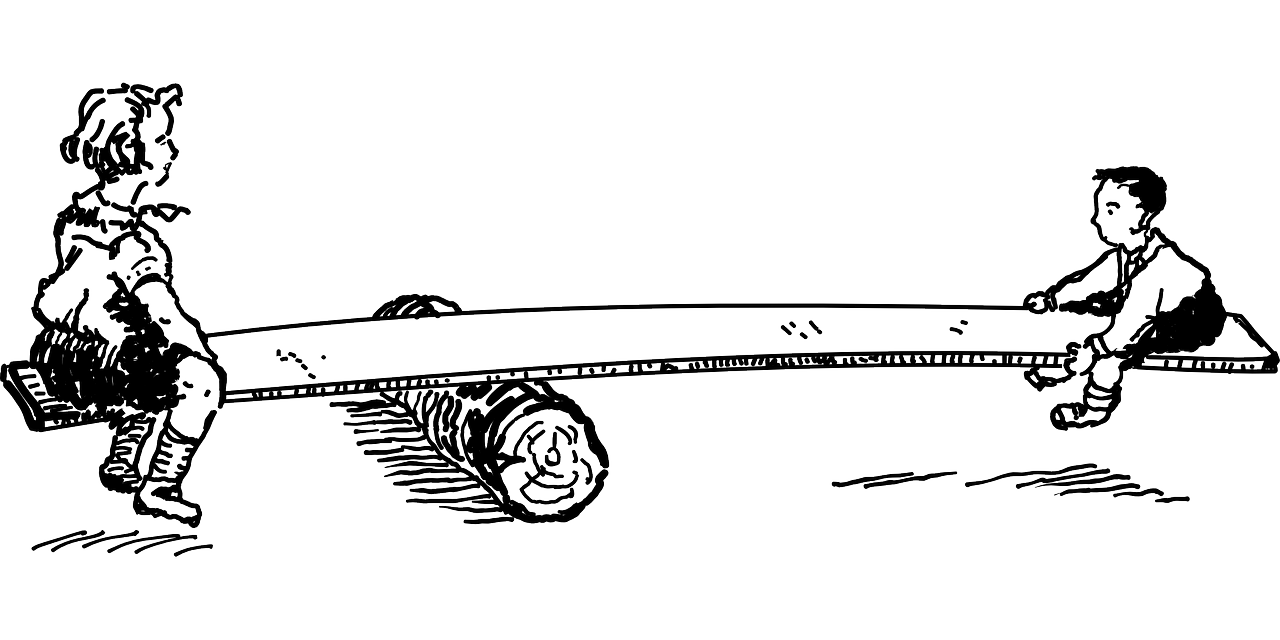
\includegraphics[scale=0.15]{../../images/teeter-totter.png}} ;
	\coordinate (C) at (2.8, -0.6);
  % \draw[blue] (-3.5,1) rectangle (3.75,-2.5);
  \only<2->{
   \draw [line width= 0.75mm,latex-, red] (B) -- +(0,-1.2) node[right] {\Large $\bm {550}\,$\bf N};
   \draw [line width= 0.75mm,-latex, red] (A) -- +(0,-1.2) node[right] {\Large $\bm {375}\,$\bf N};
   \draw [line width= 0.75mm,-latex, red] (C) -- +(0,-1.2) node[left] {\Large $\bm {175}\,$\bf N};
  }
}
		
		\end{statsbox}
		
	\end{textblock*}
\end{frame}

\begin{frame}{Why Two Equations Are Not Enough...}
	\begin{itemize}
		\item Consider a simple body, subject to two forces, equal in magnitude and opposite in direction:
	\end{itemize}

	\def\scale{0.65}
	\begin{center}
		\tcbox[colback=white,boxsep=0pt,top=15pt,bottom=15pt,left=5pt,right=5pt, enhanced, drop fuzzy shadow,colframe=structure]{
			% !TEX root = ../../Beamer/statikz/statikz.tex


\tikz[scale=\scale]{

	\coordinate (A) at (-1,0) node[above] {$A$};
	\coordinate (B) at (3,0);
	\coordinate (C) at (6, 0);

	\def\hi{0.2}
	\def\radii{0}
	\def\extend{2.5*\hi}

	% 

	\fill[white] (-3,-1.5) rectangle (7.5,1.5);

		% \pgfoonew \Beam=new beam(A,C,gray!50!white,gray!50!black,0.25,0.25,0.175)
		\Meme{A}{C}{Wheat3}{Wheat3}{black}{0.5}{0.0625}{0.125}

	\draw[ultra thick, saitRed, -Latex, line cap=round] (C) -- +(150:2)node[above] {$\bm{ F }$};
	\draw[ultra thick, saitRed, -Latex, line cap=round] (A) -- +(-30:2)node[below] {$\bm{ F }$};





}

		}
	\end{center}

	\begin{itemize}
		\item<2-> $\Sigma F_x=0$ and $\Sigma F_y=0$, but, clearly, this body is not in equilibrium; it will rotate in a counter-clockwise direction.
		\item<3-> To consider equilibrium for non-concurrent forces, {\bfseries moments} must be taken in to account.
	\end{itemize}
\end{frame}

% %%%%%%%%%%%%%%%%%%%%%%%%%%%%%%%%%%%%%%%%%%%%%%%%%%%%%%%%%%%%%%%%%%%%%%%%%%%%%%%%

\begin{frame}{Moments}
	\def\scale{0.75}
	\begin{center}
		\tcb[left=5mm, right=5mm]{
			\centering
			% !TEX root = ../../Beamer/statikz/statikz.tex


\tikz[scale=\scale]{

	\def\hi{0.1}

	\def\radii{0.05}
	\def\extend{0}

	\coordinate (A) at (-2,0);
	\coordinate (B) at (0,0);
	\coordinate (C) at (3.5,0);
	\coordinate (D) at (5.5,0);
	\coordinate (E) at (1.75,1);
  \coordinate (F) at ($ (B)!0.8!(E) $);
  \coordinate (G) at ($ (B)!0.2!(E) $);

  % \draw

	% \pgfoonew \wallA =new rr(A, B, gray!50!white,gray!50!black, 0.25)
	% \begin{scope}[opacity=0.35]
	% 	\pgfoonew \door =new rr(B, C, gray!50!white,gray!50!black, 0.25)
	% \end{scope}
	% \pgfoonew \doorB =new rr(B, E, gray!50!white,gray!50!black, 0.25)
	% \pgfoonew \wallB =new rr(C, D, gray!50!white,gray!50!black, 0.25)

	% \Meme{A}{B}{Seashell3}{Seashell3}{black}{0.25}{0.03}{0.75}
	% \Meme{B}{C}{Seashell3}{Seashell3}{black}{0.25}{0.03}{0.75}

	\filldraw[fill=Seashell3, rounded corners=0.035 cm, line width=0.25mm] ($ (A)+(0,0.125) $) rectangle ($ (B)+(0,-0.125) $);
	\filldraw[fill=Seashell3, rounded corners=0.035 cm, line width=0.25mm, opacity=0.25] ($ (B)+(0,0.125) $) rectangle ($ (C)+(0,-0.125) $);

	\filldraw[fill=Seashell3, rounded corners=0.035 cm, line width=0.25mm] ($ (B)+(120:0.125)+(0.0625,0) $) -- ++(30:3.5)--++(-60:0.25)--++(-150:3.5)--cycle;

	\filldraw[fill=Seashell3, rounded corners=0.035 cm, line width=0.25mm] ($ (C)+(0,0.125) $) rectangle ($ (D)+(0,-0.125) $);


	\node[below right] at (E) {Door};
	\fill[black] ($ (B)+(-0,0.15) $) circle (2pt) node[above left] {Hinge};
  % \draw[ultra thick, saitMaroon, latex-] (F) -- +(120:2) node [above] {$\bm{ F }$};
  % \draw[ultra thick, saitMaroon, latex-] (G) -- +(-60:2) node [below] {$\bm{ 3F $}};

	\draw[ultra thick, saitMaroon, latex-] ($ (B)+(30:3) $) -- +(120:2)node [left] {$\bm{ F }$};
	\draw[ultra thick, saitMaroon, latex-] ($ (B)+(30:1) $) -- +(-60:2)node [right] {$\bm{ 3F }$};


}

		}

	\end{center}
	\cmini[0.9]{
		\small
		Another lesson we learned as we were growing up was that is was easier to open a door by pushing or pulling on the handle that was further from the door hinges than it was to push close to the hinges.
	}

\end{frame}

% %%%%%%%%%%%%%%%%%%%%%%%%%%%%%%%%%%%%%%%%%%%%%%%%%%%%%%%%%%%%%%%%%%%%%%%%%%%%%%%%

\begin{frame}{Moments}

	\cmini[0.8]{
		\begin{statsbox}[title=Definition of a Moment]{}{%
				The {\bfseries moment} $M_O$ of a force $F$ about a point $O$ is given by:
				$$\bm{ M=Fd} $$
				where $d$ is the {\bfseries perpendicular} distance from $O$ to the line of action of the force $F$. ($d$ is known as the {\bf moment-arm}.)}
		\end{statsbox}
		\parb
		\mini[0.45]{
			\tcbox[colback=white,boxsep=0pt,top=15pt,bottom=15pt,left=5pt,right=5pt, enhanced, drop fuzzy shadow,colframe=structure]{
				\def\scale{0.3}
				\centering
				% !TEX root = ../../Beamer/statikz/statikz.tex

\tikz[scale=\scale]{

	\coordinate (O) at (0,0);
	\coordinate (A) at (1,7);
	\coordinate (B) at (4,3);
	\coordinate (C) at (7,-1);
	\coordinate (D) at (8.5,-3);
	\coordinate (E) at ($ (C)!0.8!(B) $);

	\fill[black] (O) circle (3pt) node[above left] {$O$};
	\draw (O) -- node[above] {$d$} (B);
	\draw (A) -- (D);
	\draw[line width = 0.75mm, -latex, saitMaroon, line cap=round] (C) -- (E) node [right, outer sep=2mm]{ $\bm{\mathrm{ F }}$} ;
	\draw ($ (B)+(-53.13:0.5) $) -- ++(216.87:0.5) -- +(126.87:0.5);



}

			}
		}
		\hfill
		\mini[0.5]{
			Moments are a product of force and distance so units are $\mathsf{N\cdot mm}$, $\mathsf{N\cdot m}$, $\mathsf{kN\cdot m , \, ft\cdot lb,\, in\cdot lb, \ldots} $
			\parb
			{\bfseries Sign Convention}:\lb
			If the tendency to rotate about $O$ is counter-clockwise, the moment is {\bfseries positive}. \par If clockwise, the moment is {\bfseries negative}.
		}
	}
\end{frame}


\begin{frame}

	\begin{myexam}{}{}
		\mini[0.45]{
			\centering
			\def\scale{0.6}
			% !TEX root = ../../Beamer/statikz/statikz.tex


\tikz[scale=\scale]{


	\coordinate (A) at (0,0);
	\coordinate (B) at (-2,5);

	\draw[very thick]  ($ (A)-(4,0) $) -- ($ (A)+(2,0) $);
	\Meme{A}{B}{Cornsilk3}{Cornsilk3}{black}{0.5}{0.125}{0.5}
	\fill[Cornsilk3] ($ (A)-(4,0) $) rectangle ($ (A)+(2,-1) $);

	\fill[black] (B) circle (2pt) node[left, outer sep=1.5mm, black] {$\bm B$};
	\fill[black] (A) circle (2pt) node[below, black] {$\bm A$};

	\draw[ultra thick, -latex, saitMaroon] (B) -- +(-120:3) node[below]{$3.5\,$kN};
	\draw ($ (A)+(21.8:0.5) $) -- +(21.8:1);
	\draw ($ (B)+(21.8:0.5) $) -- +(21.8:1);
	\draw[latex-latex] ($ (A)+(21.8:1) $) -- node[sloped, fill=white]{$2.30\,$m} ($ (B)+(21.8:1) $);
	\draw ($ (B)+(-68.2:1.75)  $) -- ($ (B)+(-68.2:2.75)  $);
	\draw[latex-latex] ($ (B)+(-68.2:2.2)  $) arc (-68.2:-120:2.2);
	\node[fill=white, inner sep = 0.2mm] at ($ (B)+(-95:2.15) $){\small $51.8^\circ$};




}

		}
		\hfill
		\mini[0.5]{
			Determine the moment, $M_A$, of the $3.5$ kN force applied at $B$, about the point $A$.			
		}
	\end{myexam}
\end{frame}

% %%%%%%%%%%%%%%%%%%%%%%%%%%%%%%%%%%%%%%%%%%%%%%%%%%%%%%%%%%%%%%%%%%%%%%%%%%%%%%%%

\begin{frame}

	\begin{myexam}{}{}
		\mini[0.5]{
			\def\scale{0.65}
			\parb
			% !TEX root = ../../Beamer/statikz/statikz.tex


\tikz[scale=\scale]{
	\small
	\def\hi{0.2}


	\def\extend{0.5}

	\coordinate (A) at (0,0);
	\coordinate (B) at (4,0);
	\coordinate (C) at (4,2);

	% \fill[lightgray] ($ (A)-(1,2) $) rectangle ($ (A)+(0,5) $);
	% \filldraw[fill=LightSteelBlue3, draw=black, thick] ($ (A)+(-1,2) $) -- ($ (A)-(0,2) $) -- ($ (A)+(0,-0.35) $) -- ($ (B)+(0.35,-0.35) $) -- ($ (C)+(0.35,0.5) $)  -- ($ (C)+(-0.35,0.5) $) -- ($ (B)+(-0.35,0.35) $) -- ($ (A)+(0,0.35)  $) -- ($ (A)+(0,5) $);

	\filldraw[fill=LightGoldenrod3, draw=black, thick, rounded corners=1mm] ($ (A)+(-1,4) $) -- ++(1,0) -- ++(0,-3.65) -- ($ (B)+(-0.35,0.35) $) -- ($ (C)+(-0.35,0.5) $)  -- ($ (C)+(0.35,0.5) $) -- ($ (B)+(0.35,-0.35) $)-- ($ (A)+(0,-0.35)  $)--++(0,-2)--+(-1,0);

	\draw[ultra thick, -latex, saitMaroon] (B) -- +(131:3) node[above, black] {$2.30\,$kN};
	\draw[ultra thick, -latex, saitMaroon, line cap=round] (C) -- +(90:1.5) node[above, black] {$2.05\,$kN};
	\draw[ultra thick, -latex, saitMaroon, line cap=round] (C) -- +(0:1.75) node[above, black] {$2.84\,$kN};
	\draw ($ (B)-(1.5,0) $) -- ($ (B)-(2.5,0) $);
	\draw ($ (C)+(1,0) $) -- +(1:0);

	\draw[latex-latex] ($ (B)+(131:2)  $) arc (131:180:2);

	\fill[black] (A) circle (2pt) node[left] {$\bm A$};
	\fill[black] (B) circle (2pt) node[below right, outer sep=1.25mm] {$\bm B$};
	\fill[black] (C) circle (2pt) node[xshift=0.25mm, above right, outer sep=1.25mm] {$\bm C$};
	\node[fill=white] at ($ (B)+(155:2) $){$49^\circ$};
	\draw ($ (B)+(0.5,0) $) -- +(1,0);
	\draw ($ (B)+(0,-0.5) $) -- +(0,-1);
	\draw[latex-latex] ($ (A)-(0,1) $) -- node[fill=white] {$4.00\,$m} ($ (B)-(0,1) $);
	\draw[latex-latex] ($ (C)+(1,0) $) -- node[fill=white, xshift=0.25cm] {$2.00\,$m} ($ (B)+(1,0) $);


}

		}
		\hfill
		\mini[0.4325]{
			Determine the sum of the moments of the forces, acting at $B$ and $C$, about the point $A$. \parm  Also, sum the moments of the forces about the point $B$.

		}
	\end{myexam}
\end{frame}

% %%%%%%%%%%%%%%%%%%%%%%%%%%%%%%%%%%%%%%%%%%%%%%%%%%%%%%%%%%%%%%%%%%%%%%%%%%%%%%%%

\begin{frame}{}

	\begin{myexer}{}{}
		\def\scale{0.65}
		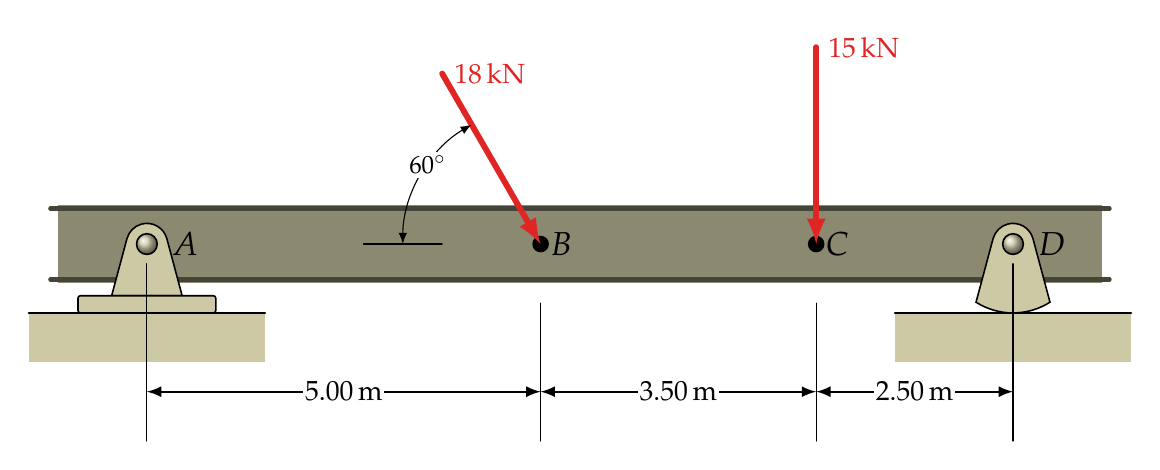
\begin{tikzpicture}[scale=\scale, line cap=round]
	\def\thickness{thick}
	\def\stroke{black}
	\def\hi{.4}
	\def\radii{0}
	\def\extend{3*\hi}
	\def\nuhi{0.45}
	\def\nuext{1.225}

	\coordinate (A) at (0, 0);
	\coordinate (B) at (5, 0);
	\coordinate (C) at (8.5, 0);
	\coordinate (D) at (11, 0);

	\fill[LemonChiffon4] ($ (A)+(-1.125,0.5) $) rectangle ($ (D)+(1.125,-0.5) $);

	\fill[LemonChiffon3] ($ (A)-(1.5,0.875) $) rectangle ($ (A)+(1.5,-1.5) $);
	\fill[LemonChiffon3] ($ (D)-(1.5,0.875) $) rectangle ($ (D)+(1.5,-1.5) $);
	\draw[thick] ($ (A)-(1.5,0.875) $) -- ($ (A)+(1.5,-0.875) $);
	\draw[thick] ($ (D)-(1.5,0.875) $) -- ($ (D)+(1.5,-0.875) $);

	\draw[ultra thick, LemonChiffon4!50!black] ($ (A)+(-\nuext, \nuhi) $) -- ($ (D)+(\nuext, \nuhi) $);
	\draw[ultra thick, LemonChiffon4!50!black] ($ (A)+(-\nuext, -\nuhi) $) -- ($ (D)+(\nuext, -\nuhi) $);
	

	\fill[black] (A) circle (3pt) node[xshift=1mm, right, outer sep=1mm] {\large $A$};
	\fill[black] (B) circle (3pt) node[right] {\large $B$};
	\fill[black] (C) circle (3pt) node[right] {\large $C$};
	\fill[black] (D) circle (3pt) node[xshift=1mm,right, outer sep=1mm] {\large $D$};

	\PC{A}{LemonChiffon3}{black}{0.875}{0.2}
	\Rocker{D}{LemonChiffon3}{black}{0.875}{0.2}


	\draw ($ (B)+(0,-0.75) $) -- +(0,-1.752);
	\draw ($ (A)+(0,-0.25) $) -- +(0,-2.252);
	\draw ($ (C)+(0,-0.75) $) -- +(0,-1.752);
	\draw ($ (D)+(0,-0.25) $) -- +(0,-2.252);

	\draw[thick, latex-latex] ([yshift=-1.875cm]A) -- node[fill=white, inner sep= 0.2mm]{$5.00\,$m}([yshift=-1.875cm]B);
	\draw[thick, latex-latex] ([yshift=-1.875cm]B) -- node[fill=white, inner sep= 0.2mm]{$3.50\,$m}([yshift=-1.875cm]C);
	\draw[thick, latex-latex] ([yshift=-1.875cm]C) -- node[fill=white, inner sep= 0.2mm]{$2.50\,$m}([yshift=-1.875cm]D);

	\draw ($ (B)-(1.25,0) $) -- +(-1,0);

	\draw[line width=0.75mm, saitRed, latex-] (C) -- +(0,2.5) node[right] { $15\,$kN};
	\draw[line width=0.75mm, saitRed, latex-] (B) -- ($ (B) + (120:2.5) $) node[right] {$18\,$kN};

	\draw[latex-latex] ($ (B)+(180:1.75)  $)  arc (180:120:1.75);
	\path ($ (B)+(145:1.75) $) node[fill=white, inner sep=0.5mm] {\small $60\deg$};

\end{tikzpicture}

		\cmini[0.9]{
			Rigid beam $ABCD$ is supported at $A$ and at $D$, and is subjected to the two forces shown at $B$ and $C$.\parm
			Determine the value of the reaction at $D$, $R_D$, if the sum of the moments about $A$, $\Sigma M_A$, is zero and the reaction at $D$ is vertically upwards.
		}
	\end{myexer}
\end{frame}

% %%%%%%%%%%%%%%%%%%%%%%%%%%%%%%%%%%%%%%%%%%%%%%%%%%%%%%%%%%%%%%%%%%%%%%%%%%%%%%%%

\begin{frame}{The Principle of Moments}
	The Principle of Moments,  often referred to as Varignon's Theorem, is stated~below:\parm
	\begin{statsbox}[title=Varignon's Theorem, left=5mm, right=5mm]
		\centering
		The moment of a force about a point  is equal to the sum of the moments of the components of the force about the same point.
	\end{statsbox}
	\parb
	In many cases, it is more convenient to sum the moments of a forces components than it is to use the formula directly.

	There are two primary ways we use this result:
	\begin{itemize}
		\item Resolve the force into horizontal and vertical components
		\item Resolve the force into orthogonal (perpendicular to each other) components, with the line of action of one component passing through the point about which we are taking moments -- so that its moment is zero ($d=0$).
	\end{itemize}

	% \cmini[0.8]{
	% 	\footnotesize
	% 	\textcolor{saitMaroon}{(Another Varignon's Theorem, attributed to the same French mathematician, is a delightful result for those interested in geometry: the midpoints of the sides of any quadrilateral (four-sided polygon) form the vertices of a parallelogram. Furthermore, the area of the parallelogram is half that of the quadrilateral! :)}
	% }
\end{frame}

% %%%%%%%%%%%%%%%%%%%%%%%%%%%%%%%%%%%%%%%%%%%%%%%%%%%%%%%%%%%%%%%%%%%%%%%%%%%%%%%

% \begin{frame}{}
% 	\begin{myexam}{}{}
% 		\def\scale{0.75}
% 		% !TEX root = ../../Beamer/statikz/statikz.tex

\makeatletter
\providecommand{\gettikzxy}[3]{%
	\tikz@scan@one@point\pgfutil@firstofone#1\relax
	\edef#2{\the\pgf@x}%
	\edef#3{\the\pgf@y}%
}
\makeatother

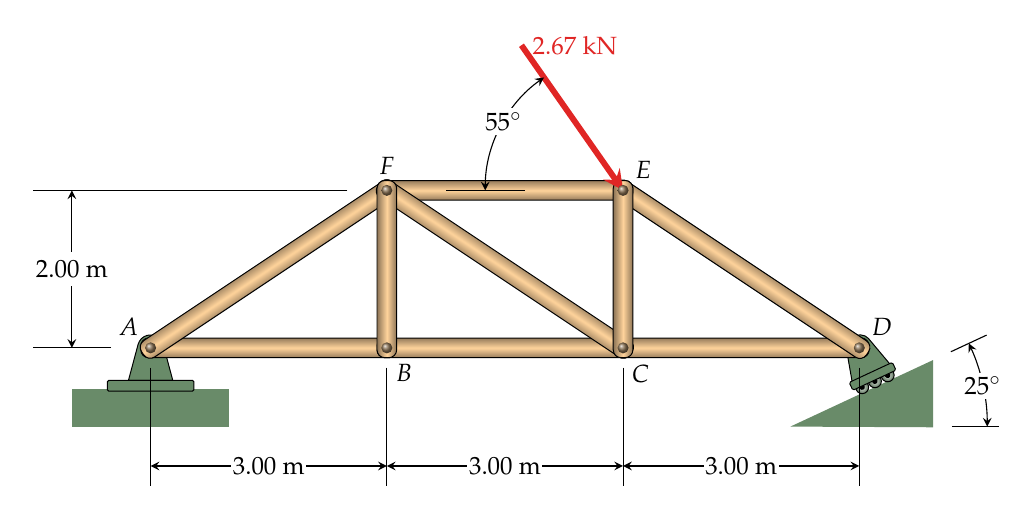
\begin{tikzpicture}[scale=\scale]
	\def\thickness{thick}
	% \def\stroke{black}
	\def\hi{.15}
	\def\radii{\hi}
	\def\extend{\hi}
	\small

	\coordinate (A) at (0, 0);
	\coordinate (B) at (3, 0);
	\coordinate (C) at (6, 0);
	\coordinate (D) at (9, 0);
	\coordinate (E) at (6, 2);
	\coordinate (F) at (3, 2);
	\coordinate (AA) at ($ (A)+(0,-0.5) $);

	\gettikzxy{(AA)}{\aax}{\aay}

	\fill[DarkSeaGreen4] ($ (A)-(1,0.525) $) rectangle ($ (A)+(1,-1) $);
	\fill[DarkSeaGreen4] ($ (D)+(-0.875,-1) $) -- ++(25:2) -- +(-90:0.854) -- cycle;

	\PC{A}{DarkSeaGreen4}{black}{0.55}{0.125}
	\Roller[25]{D}{DarkSeaGreen4}{black}{0.55}{0.125}

	\draw ($ (A)+(0,-0.25) $) -- +(0,-1.5);
	\draw ($ (B)+(0,-0.25) $) -- +(0,-1.5);
	\draw ($ (C)+(0,-0.25) $) -- +(0,-1.5);
	\draw ($ (D)+(0,-0.25) $) -- +(0,-1.5);

	\Meme{A}{B}{Burlywood4}{Burlywood1}{black}{0.25}{0.1}{0.125};
	\Meme{B}{C}{Burlywood4}{Burlywood1}{black}{0.25}{0.1}{0.125};
	\Meme{D}{C}{Burlywood4}{Burlywood1}{black}{0.25}{0.1}{0.125};
	\Meme{D}{E}{Burlywood4}{Burlywood1}{black}{0.25}{0.1}{0.125};
	\Meme{F}{E}{Burlywood4}{Burlywood1}{black}{0.25}{0.1}{0.125};
	\Meme{F}{A}{Burlywood4}{Burlywood1}{black}{0.25}{0.1}{0.125};
	\Meme{F}{C}{Burlywood4}{Burlywood1}{black}{0.25}{0.1}{0.125};
	\Meme{F}{B}{Burlywood4}{Burlywood1}{black}{0.25}{0.1}{0.125};
	\Meme{C}{E}{Burlywood4}{Burlywood1}{black}{0.25}{0.1}{0.125};




	% \draw ($ (B)+(0,-0.75) $) -- +(0,-1.752);
	% \draw[line width=0.75mm, red, ->, >=stealth] (C) -- +(0,-2.5) node[below] { 15 kN};
	% \draw[line width=0.75mm, red, <-, >=stealth] ($ (D)$) -- +(-90:2.25) node[below] {$\bm{\mathrm{ R }_{D}}$};
	% \draw[line width=0.75mm, red, <-, >=stealth] ($ (A)$) -- +(-90:2.25) node[below] {$\bm{\mathrm{ R }_{A_y}}$};
	\draw[line width=0.75mm, saitRed, <-, >=stealth] (E) -- +(125:2.25) node[right] {2.67 kN};
	\draw ($ (E)+(-1.25,0) $)  -- ($ (E)+(-2.25,0) $);
	\draw[<->, >=stealth] ($ (E)+(-1.75,0) $)  arc (180:125:1.75);
	\path  ($ (E)+(150:1.75) $) node[fill=white, inner sep=0.5mm] {\small $55^\circ$};

	\draw ($ (A)-(0.5, 0) $) -- ($ (A)-(1.5, 0) $);
	\draw ($ (F)-(0.5, 0) $) -- ($ (F)-(4.5, 0) $);
	\draw[ <->, >=stealth] ($ (A)-(1, 0) $) -- node[fill=white, outer sep= 0.2mm]{2.00 m}($ (F)-(4, 0) $);

	\draw[ <->, >=stealth] ([yshift=-1.5cm]A) -- node[fill=white, inner sep= 0.2mm]{3.00 m}([yshift=-1.5cm]B);
	\draw[ <->, >=stealth] ([yshift=-1.5cm]B) -- node[fill=white, inner sep= 0.2mm]{3.00 m}([yshift=-1.5cm]C);
	\draw[ <->, >=stealth] ([yshift=-1.5cm]C) -- node[fill=white, inner sep= 0.2mm]{3.00 m}([yshift=-1.5cm]D);

	 \draw ($ (D)+(-0.875,-1)+(25:2.25) $) -- +(25:0.5);
	  \draw ($ (D)+(-0.875,-1)+(0:2.05) $) -- +(0:0.6);
	 \draw[<->, >=stealth] ($ (D)+(-0.875,-1)+(0:2.5) $)  arc (0:25:2.5);
	 \path  ($ (D)+(-0.875,-1)+(12:2.5) $) node[fill=white, inner sep=0.5mm] {\small $25^\circ$};

	\shade[ball color=Burlywood4] (A) circle (2pt) node[above left, outer sep=0.5mm] {$A$};
	\shade[ball color=Burlywood4] (B) circle (2pt) node[below right, yshift=-1mm] {$B$};
	\shade[ball color=Burlywood4] (C) circle (2pt) node[below right, yshift=-1mm] {$C$};
	\shade[ball color=Burlywood4] (D) circle (2pt) node[above right, outer sep=0.5mm] {$D$};
	\shade[ball color=Burlywood4] (E) circle (2pt) node[above right, outer sep=0.5mm] {$E$};
	\shade[ball color=Burlywood4] (F) circle (2pt) node[yshift=0.5mm, above, outer sep=0.5mm] {$F$};




\end{tikzpicture}

% 		\cmini[0.9]{
% 			The truss shown is supported by a pinned connection at $A$ and a roller (on a plane inclined at $25^\circ$ to the horizontal) at $D$. Determine the magnitude and direction of $R_D$, the reaction at $D$, if the sum of the moments about $A$ is zero.
% 		}
% 		% \begin{center}
% 		% 	\footnotesize
% 		% 	\rotatebox[origin=c]{180}{
% 		% 		\textcolor{gray}{
% 		% 			($R_D=1.98\,\mathsf{kN}$)
% 		% 		}
% 		% 	}
% 		% \end{center}

% 	\end{myexam}
% \end{frame}




%%%%%%%%%%%%%%%%%%%%%%%%%%%%%%%%%%%%%%%%%%%%%%%%%%%%%%%%%%%%%%%%%%%%%%%%%%%%%%%%

\begin{frame}
	\cmini{
		\begin{myexam}{}{}
			\centering\parb
			\tikz[scale=\scale]{

	\coordinate (A) at (0,0);
	\coordinate (B) at (5,0);

  \fill[LightSteelBlue3, rounded corners=5mm] ($ (A)+(0,1.5) $) to [out=225, in=135] ($ (A)-(0,1.5) $);
  % \fill[Sienna3] (($ (A)+(0,1) $) rectangle ($ (A)+(0,-3) $);)
  \draw[semithick] ($ (A)+(0,1.5) $) -- ($ (A)+(0,-1.5) $);
  \Meme{A}{B}{SlateGray4}{SlateGray1}{SlateGray3}{0.5}{0}{0.1}
  \draw[line width= 0.5mm, line cap=round] ($ (A)+(-0.25,0.25) $) --  ($ (B)+(0.25,0.25) $);
  \draw[line width= 0.5mm, line cap=round] ($ (A)+(-0.25,-0.25) $) --  ($ (B)+(0.25,-0.25) $);

  \draw[ultra thick, saitRed, -latex] (B) -- +(-63:2) node[below] {$3.00\,$kN};
  \fill (A) circle (2pt) node[right] {$A$};
  \fill (B) circle (2pt) node[left] {$B$};

  \draw ($ (B)+(0,0.5) $) -- +(0,0.5);
  \draw[latex-latex] ($ (A)+(0,0.75) $) -- node[midway, fill=white] {$3.00\,$m} ($ (B)+(0,0.75) $);
  \draw ($ (B)+(0.5,0) $) -- +(1,0);
  \draw[latex-latex] ($ (B)+(1,0) $)  arc(0:-63:1) node[midway, fill=white, inner sep=0.3mm] {$63\deg$};

  % \draw[gray]


}

			\parb
			Determine the moment about $A$ of the force applied to $B$ by resolving the force at $B$ into horizontal and vertical components.
		\end{myexam}
	}
\end{frame}

%%%%%%%%%%%%%%%%%%%%%%%%%%%%%%%%%%%%%%%%%%%%%%%%%%%%%%%%%%%%%%%%%%%%%%%%%%%%%%%%

\begin{frame}
	\cmini[1]{
		\begin{myexam}{}{}
			\def\scale{0.6}
			\centering
			% !TEX root = ../../Beamer/statikz/statikz.tex


\tikz[scale=\scale]{


	\coordinate (A) at (0,0);
	\coordinate (B) at (-2,5);

	\draw[very thick]  ($ (A)-(4,0) $) -- ($ (A)+(2,0) $);
	\Meme{A}{B}{Cornsilk3}{Cornsilk3}{black}{0.5}{0.125}{0.5}
	\fill[Cornsilk3] ($ (A)-(4,0) $) rectangle ($ (A)+(2,-1) $);

	\fill[black] (B) circle (2pt) node[left, outer sep=1.5mm, black] {$\bm B$};
	\fill[black] (A) circle (2pt) node[below, black] {$\bm A$};

	\draw[ultra thick, -latex, saitMaroon] (B) -- +(-120:3) node[below]{$3.5\,$kN};
	\draw ($ (A)+(21.8:0.5) $) -- +(21.8:1);
	\draw ($ (B)+(21.8:0.5) $) -- +(21.8:1);
	\draw[latex-latex] ($ (A)+(21.8:1) $) -- node[sloped, fill=white]{$2.30\,$m} ($ (B)+(21.8:1) $);
	\draw ($ (B)+(-68.2:1.75)  $) -- ($ (B)+(-68.2:2.75)  $);
	\draw[latex-latex] ($ (B)+(-68.2:2.2)  $) arc (-68.2:-120:2.2);
	\node[fill=white, inner sep = 0.2mm] at ($ (B)+(-95:2.15) $){\small $51.8^\circ$};




}

			\parm
			\raggedright
			
			\ccbox[0.8]{Cornsilk3}{Cornsilk3}{\small (Revisiting {\itshape\rmfamily Example 1}.) Notice that we cannot calculate the moment about $A$ of the force acting on $B$ using horizontal and vertical components because, without the angle at which $AB$ is inclined, we cannot determine the moment arm, $d$, for either the horizontal or the vertical component.} 
			\parm\centering
			Determine the moment about $A$ of the force at $B$ by resolving the force into components parallel to and perpendicular to $AB$.
		\end{myexam}
	}
\end{frame}

%%%%%%%%%%%%%%%%%%%%%%%%%%%%%%%%%%%%%%%%%%%%%%%%%%%%%%%%%%%%%%%%%%%%%%%%%%%%%%%%

\begin{frame}
	\cmini[1]{
		\begin{myexer}{}{}
			\def\scale{0.8}
			\centering\parb
			\tikz[scale=\scale]{

	\coordinate (A) at (0,0);
	\coordinate (B) at (-6,0);
	\coordinate (Ddown) at (-5.625,-0.625);

  \fill[Snow3] ($ (A)+(0,1.5) $) to [out=-15, in=15] ($ (A)-(0,1.5) $);
  \EyeBolt[180]{Ddown}{Snow3}{black}{0.5}{0.5}
  \draw[semithick] ($ (A)+(0,1.5) $) -- ($ (A)+(0,-1.5) $);
  \Meme{A}{B}{Snow4}{Snow1}{Snow3}{0.5}{0}{0.1}
  \draw[line width= 0.5mm, line cap=round] ($ (A)+(0.25,0.25) $) --  ($ (B)+(-0.25,0.25) $);
  \draw[line width= 0.5mm, line cap=round] ($ (A)+(0.25,-0.25) $) --  ($ (B)+(-0.25,-0.25) $);

  

  \draw[ultra thick, black, -latex] (Ddown) -- +(222:2.25) node[below] {$960\,$N};
  \fill (A) circle (2pt) node[left] {$A$};
  \fill ($  (Ddown)+(0,0.625)  $) circle (2pt) node[left] {$B$};
  % \node[below right] at (Ddown) {$B$};
  \node[below right] at (Ddown) {$C$};

  \draw ($ (Ddown)+(0,1.125) $) -- +(0,0.5);
  \draw[latex-latex] ($ (A)+(0,0.75) $) -- node[midway, fill=white] {\small $2.15\,$m} ($ (Ddown)+(0,1.375) $);
  \draw ($ (Ddown)+(0.25,0) $) -- +(1.5,0);
  \draw[latex-latex] ($ (Ddown)+(-1.5,0) $)  arc(180:222:1.5) node[midway, fill=white, inner sep=0.3mm] {\small $42\deg$};
  \draw ($ (B)-(0.5,0) $) -- +(-1,0);
  \draw ($ (Ddown)-(0.25,0) $) -- +(-1.625,0);
  \draw[latex-latex] ($ (Ddown)+(-1.5,0) $) -- node[midway, fill=white, inner sep=0mm]{\footnotesize $140\,$mm} +(0,0.625)

  % \draw[gray]


}

			\parm	
			Determine the moment about $A$ of the force acting at $C$. \lb Then determine the moment about $B$ for the same force.
		\end{myexer}
	}
\end{frame}

%%%%%%%%%%%%%%%%%%%%%%%%%%%%%%%%%%%%%%%%%%%%%%%%%%%%%%%%%%%%%%%%%%%%%%%%%%%%%%%%

\begin{frame}
	\cmini[1]{
		\begin{myexer}{}{}
			\def\scale{0.8}
			\centering
			\tikz[scale=\scale]{

	\coordinate (A) at (0,0);
	\coordinate (B) at (2.5,0);
	\coordinate (C) at (5,0);
	\coordinate (D) at (7,0);
	\coordinate (Dd) at (7,-1);
	\coordinate (Du) at (7,1);


  \EyeBolt[180]{Dd}{Seashell2}{black}{0.5}{0.75}
  \EyeBolt{Du}{Seashell2}{black}{0.5}{0.75}
  \filldraw[fill=Seashell2, draw=black, rounded corners=0.75mm, line width=0.325mm ] ($ (A)+(-1,-3) $) -- ($ (A)+(0,-3) $) -- ($ (A)+(0,-0.25) $) -- ($ (D)+(0.65,-0.25) $) -- +(0,0.5) -- ($ (A)+(0,0.25) $) -- ($ (A)+(0,2) $) -- ($ (A)+(-1,2) $);

  \fill (A) circle (2pt) node[left] {$A$};
  \fill (B) circle (2pt) node[left] {$B$};
  \fill (C) circle (2pt) node[right] {$C$};
  \fill (D) circle (2pt) node[right] {$D$};

  \draw[very thick, statsRed, -latex] (B) -- +(65:1.5) node[above] {$1020\,$N};
  \draw[very thick, statsRed, -latex] (C) -- +(245:1.5) node[left] {$1020\,$N};
  \draw[very thick, statsRed, -latex] (Du) -- +(180:1.75) node[left] {$1690\,$N};
  \draw[very thick, statsRed, -latex] (Dd) -- +(0:1.75) node[right] {$1690\,$N};

	\draw ($ (B)+(0.25,0) $) -- ($ (C)+(-0.25,0) $);
  \draw[latex-latex] ($ (B)+(1,0) $)  arc(0:65:1) node[midway, fill=white, inner sep=0.3mm] {\small $65\deg$};
  \draw[latex-latex] ($ (C)+(-1,0) $)  arc(180:245:1) node[midway, fill=white, inner sep=0.3mm] {\small $65\deg$};
  
  \draw ($ (Du)+(0.5,0) $) --+ (1.5,0);
  \draw[latex-latex] ($ (Du)+(1.25,0) $) -- ($ (Dd)+(1.25,0) $) node[midway, fill=white, xshift=0.25cm] {\small $600\,$mm};

  \draw ($ (D)+(0,-1.25) $) -- ($ (D)+(0,-2.5) $);
  \draw ($ (C)+(0,-.5) $) -- ($ (C)+(0,-2.5) $);
  \draw ($ (B)+(0,-.5) $) -- ($ (B)+(0,-2.5) $);

  \draw[latex-latex] ($ (A)+(0, -2) $) -- ($ (B)+(0, -2) $) node[midway, fill=white] {\small $750\,$mm};
  \draw[latex-latex] ($ (B)+(0, -2) $) -- ($ (C)+(0, -2) $) node[midway, fill=white] {\small $750\,$mm};
  \draw[latex-latex] ($ (C)+(0, -2) $) -- ($ (D)+(0, -2) $) node[midway, fill=white] {\small $600\,$mm};


}

			\parm	
			\cmini[0.7]{
				\centering
				Determine the sum of the moments about $A$, about $C$ and about $F$, of the forces shown.
			}
			
		\end{myexer}
	}
\end{frame}

% %%%%%%%%%%%%%%%%%%%%%%%%%%%%%%%%%%%%%%%%%%%%%%%%%%%%%%%%%%%%%%%%%%%%%%%%%%%%%%%%

\begin{frame}{Moments of Force Couples}
	\cmini[0.9]{
		\begin{itemize}
			\item  In the previous exercise, we found that the moments were the same about any of the points used.
			\item 	Also, the forces are different: there is an equal and opposite pair with magnitude $1690\,$N and an equal and opposite pair with magnitude $1020\,$N.
			\item Such pairs of forces, with parallel lines of action, equal magnitude and opposite sense are called force {\bfseries couples}.
			\item The resultant force of a couple is zero: $\Sigma F_x=0$ and $\Sigma F_y=0$.
			\item The {\bfseries moment of a couple}, irrespective of any point, has magnitude
			      \cmini[0.6]{
			      	\begin{statsbox}{A Couple Defined:}
			      		$$ M=F\cd d $$
			      		\centering
								\cmini{
									\centering
									where $d$ is the distance between the two lines of action.
								}
			      		
			      	\end{statsbox}
			      }
			\item Clockwise couples are considered negative, counter-clockwise couples are considered positive.
		\end{itemize}
	}
\end{frame}

% %%%%%%%%%%%%%%%%%%%%%%%%%%%%%%%%%%%%%%%%%%%%%%%%%%%%%%%%%%%%%%%%%%%%%%%%%%%%%%%%

\begin{frame}
		\begin{myexam}{}{}
			\centering
			\def\scale{0.8}
			\parb
			\tikz[scale=\scale]{

	\coordinate (A) at (0,0);
	\coordinate (B) at (2.5,0);
	\coordinate (C) at (5,0);
	\coordinate (D) at (7,0);
	\coordinate (Dd) at (7,-1);
	\coordinate (Du) at (7,1);


  \EyeBolt[180]{Dd}{Seashell2}{black}{0.5}{0.75}
  \EyeBolt{Du}{Seashell2}{black}{0.5}{0.75}
  \filldraw[fill=Seashell2, draw=black, rounded corners=0.75mm, line width=0.325mm ] ($ (A)+(-1,-3) $) -- ($ (A)+(0,-3) $) -- ($ (A)+(0,-0.25) $) -- ($ (D)+(0.65,-0.25) $) -- +(0,0.5) -- ($ (A)+(0,0.25) $) -- ($ (A)+(0,2) $) -- ($ (A)+(-1,2) $);

  \fill (A) circle (2pt) node[left] {$A$};
  \fill (B) circle (2pt) node[left] {$B$};
  \fill (C) circle (2pt) node[right] {$C$};
  \fill (D) circle (2pt) node[right] {$D$};

  \draw[very thick, statsRed, -latex] (B) -- +(65:1.5) node[above] {$1020\,$N};
  \draw[very thick, statsRed, -latex] (C) -- +(245:1.5) node[left] {$1020\,$N};
  \draw[very thick, statsRed, -latex] (Du) -- +(180:1.75) node[left] {$1690\,$N};
  \draw[very thick, statsRed, -latex] (Dd) -- +(0:1.75) node[right] {$1690\,$N};

	\draw ($ (B)+(0.25,0) $) -- ($ (C)+(-0.25,0) $);
  \draw[latex-latex] ($ (B)+(1,0) $)  arc(0:65:1) node[midway, fill=white, inner sep=0.3mm] {\small $65\deg$};
  \draw[latex-latex] ($ (C)+(-1,0) $)  arc(180:245:1) node[midway, fill=white, inner sep=0.3mm] {\small $65\deg$};
  
  \draw ($ (Du)+(0.5,0) $) --+ (1.5,0);
  \draw[latex-latex] ($ (Du)+(1.25,0) $) -- ($ (Dd)+(1.25,0) $) node[midway, fill=white, xshift=0.25cm] {\small $600\,$mm};

  \draw ($ (D)+(0,-1.25) $) -- ($ (D)+(0,-2.5) $);
  \draw ($ (C)+(0,-.5) $) -- ($ (C)+(0,-2.5) $);
  \draw ($ (B)+(0,-.5) $) -- ($ (B)+(0,-2.5) $);

  \draw[latex-latex] ($ (A)+(0, -2) $) -- ($ (B)+(0, -2) $) node[midway, fill=white] {\small $750\,$mm};
  \draw[latex-latex] ($ (B)+(0, -2) $) -- ($ (C)+(0, -2) $) node[midway, fill=white] {\small $750\,$mm};
  \draw[latex-latex] ($ (C)+(0, -2) $) -- ($ (D)+(0, -2) $) node[midway, fill=white] {\small $600\,$mm};


}

			\parm
			Determine $\Sigma M$, the sum of the moments, of the couples shown.
		\end{myexam}
\end{frame}

% %%%%%%%%%%%%%%%%%%%%%%%%%%%%%%%%%%%%%%%%%%%%%%%%%%%%%%%%%%%%%%%%%%%%%%%%%%%%%%%%

\begin{frame}

	\begin{myexam}{}{}
		\def\scale{0.5}
		\begin{center}
			% !TEX root = ../../Beamer/05Moments/05Moments.tex


\begin{tikzpicture}[scale=\scale]
	\def\thickness{thick}
	\def\stroke{black}
	\def\hi{.4}
	\def\radii{0.5*\hi}
	\def\extend{3*\hi}
	\def\nuhi{0.45}
	\def\nuext{1.25}

	\coordinate (A) at (0, 0);
	\coordinate (D) at (11, 1);
	\coordinate (B) at ($ (A)!0.25!(D) $);
	\coordinate (C) at ($ (A)!0.667!(D) $);

	\fill[Cornsilk3] ($ (A)-(1.5,1.125) $) rectangle ($ (A)+(1.5,-1.5) $);
	\fill[Cornsilk3] ($ (D)-(1.5,1.125) $) rectangle ($ (D)+(1.5,-1.5) $);

	\Meme{A}{D}{Burlywood3}{Burlywood3}{black}{1}{0.1}{0.75}

	\fill[black] (A) circle (3pt) node[above, outer sep=2mm] {$A$};
	\fill[black] (B) circle (3pt) ;
	\fill[black] (C) circle (3pt);
	\fill[black] (D) circle (3pt) node[above, outer sep=2mm] {$B$};

	\PC{A}{Cornsilk3}{black}{1.125}{0.25}
	\Rocker{D}{Cornsilk3}{black}{1.125}{0.25}
	\Couple{B}{Blue3}{1}{0.75}
	\Couple[0]{C}{Blue3}{1}{0.75}

	\node[yshift=0.75cm] at (B) {\small $18.00\mathsf{\;kN\cd m}$};
	\node[yshift=0.75cm] at (C) {\small $23.00\mathsf{\;kN\cd m}$};

	% \draw[->, >=stealth, blue, ultra thick] ($ (B)+(60:0.875) $) node[black, above, outer sep=1mm]{\small $18.00\mathsf{\;kN\cdot m}$} arc (60:360:0.875)-- +(90:0.375);
	% \draw[->, >=stealth, blue, ultra thick] ($ (C)+(330:0.875) $) node[black, below, outer sep=3mm]{\small $23.0\mathsf{\;kN\cdot m}$} arc (330:30:0.875)-- +(-65:0.375);

	\draw ($ (A)+(0,-0.75) $) -- +(0,-1.752);
	\draw ($ (D)+(0,-0.75) $) --  +(0,-2.752);

	\draw[thick, <->, >=stealth] ([yshift=-1.875cm]A) -- node[fill=white, inner sep= 0.2mm]{\small $3.00\,$m}([yshift=-2.875cm]D);

	\draw[latex-, statsRed, ultra thick] (D) -- +(0,-2.25) node[right] {$R_{B}$};
	\draw[latex-, statsRed, ultra thick] (A) -- +(0,-2.5) node[left] {$R_{Ay}$};
	\draw[latex-, statsRed, ultra thick] (A) -- +(-2.25,0) node[above] {$R_{Ax}$};



\end{tikzpicture}

		\end{center}
		\cmini[0.7]{
			\parb
			Considering beam $AB$:
			\begin{enumerate}
				\item Determine the magnitude of $R_D$ if $\Sigma M_A=0$.
				\item Determine the magnitude of $R_{Ay}$ if $\Sigma F_y=0$.
				\item Determine the magnitude of $R_{Ax}$ if $\Sigma F_x=0$.
			\end{enumerate}
			
		}
	\end{myexam}
\end{frame}
% %%%%%%%%%%%%%%%%%%%%%%%%%%%%%%%%%%%%%%%%%%%%%%%%%%%%%%%%%%%%%%%%%%%%%%%%%%%%%%%%

\begin{frame}

	\begin{myexer}{}{}
		\def\scale{0.5}
		\begin{center}
			% !TEX root = ../../Beamer/05Moments/05Moments.tex


\begin{tikzpicture}[scale=\scale]


	\coordinate (A) at (0, 0);
	\coordinate (C) at (10, 0);
	\coordinate (D) at ($(C)+(0,1.25)$);
	\coordinate (B) at ($ (A)!0.75!(C) $);
  \filldraw[fill=Ivory3, draw=black, thick, rounded corners] ($ (C)+(0.25,0) $) rectangle ($ (C)+(-0.25,1.5) $);
	\Meme{A}{C}{Ivory3}{Ivory3}{black}{0.875}{0.1}{0.75}  

	\fill[black] (A) circle (3pt) node[right, xshift=1mm] {$A$};
	\fill[black] (C) circle (3pt)node[left] {$C$};
	\fill[black] (B) circle (3pt) node[left] {$B$};
	\fill[black] (D) circle (3pt) node[left, xshift=-0.5mm] {$D$};

  \fill[Ivory4] ($ (A)+(-0.875,2.5) $) to [out=180, in=180] ($ (A)+(-0.875,-2.5) $);
  \draw[thick] ($ (A)+(-0.875,2.5) $) -- ($ (A)+(-0.875,-2.5) $);

	\PC[270]{A}{Ivory4}{black}{0.875}{0.25}
	\Couple[0]{B}{statsMaroon}{1}{0.75}
	\node[yshift=0.75cm, xshift=-0.5cm] at (B) {\small $1450\mathsf{\;N\cd m}$};

  \draw[ultra thick, statsMaroon, -latex] (D) --+ (78:3) node[left, black] {$ T $};

	\draw ($ (C)+(0.75,0) $) -- +(2.25,0);
	\draw ($ (D)+(0.5,0) $) --  +(2.5,0);

	\draw[latex-latex] ($ (D)+(2,0) $)  arc(0:78:2)  node[midway, fill=white, inner sep=0.5mm] {\small $78\deg$};
	\draw[latex-latex] ($ (D)+(2,0) $)  --  node[midway, fill=white, inner sep=0mm] {\small $200\,$mm} ($ (C)+(2,0) $); 

  \draw ($ (A)+(0,-0.75) $) -- +(0, -1.5);
	\draw ($ (C)+(0,-0.75) $) --  +(0, -1.5);

  \draw[latex-latex] ($ (A)+(0,-1.75) $)  --  node[midway, fill=white, inner sep=1mm] {\small $1200\,$mm} ($ (C)+(0,-1.75) $); 


\end{tikzpicture}

		\end{center}
		\cmini[0.8]{
			\parb
			$ABCD$ has a negative couple applied at $B$ and is supported by a cable at $D$. 
			\begin{enumerate}
				\item Determine the magnitude of $T$ if $\Sigma M_A=0$.
				\item Determine the reaction at $A$ if $\Sigma F_x = \Sigma F_y =0$.				
			\end{enumerate}
			
		}
	\end{myexer}
\end{frame}

% %%%%%%%%%%%%%%%%%%%%%%%%%%%%%%%%%%%%%%%%%%%%%%%%%%%%%%%%%%%%%%%%%%%%%%%%%%%%%%%%


\begin{frame}{Distributed Loads}

	\begin{textblock*}{1\textwidth}(1cm, 1.25cm)
		\begin{tcolorbox}[colback=white,colframe=structure,top=0pt, bottom=5pt, enhanced, drop fuzzy shadow]
			\tikz{
	\coordinate (A) at (-2,0);
	\coordinate (B) at (4,0);
	\coordinate (C) at (6, 0);
	% beams
	\coordinate (D) at (0,0.41);
	\coordinate (E) at (6,0.41);
	\coordinate (F) at (0,0.705);
	\coordinate (G) at (6,0.705);
	\coordinate (H) at (0,1);
	\coordinate (I) at (6,1);

	% \def\hi{0.2}
	% \def\radii{0}
	% \def\extend{0.75}

	% \def\whi{0.15};
	\coordinate (J) at ($ (H)+ (-0.125, 0.125)$);
	\coordinate (K) at ($ (I)+ (0.125,0.125)$);
	\coordinate (L) at ($ (C)+ (0, 0.255)$);
	\coordinate (Dtriangular) at ($ (D)+ (-0.125, -0.125)$);

	\fill[white] (-3,-1.5) rectangle (7,1.75);
	\fill[Honeydew3] (-3,-1.5) rectangle (6.75,-0.6);
	\draw[thick] (-3,-0.6) -- (6.75,-0.6);

	\Meme{A}{C}{Snow3}{Snow3}{black}{0.5}{0.1}{0.75}
	\PC{A}{Honeydew4}{black}{0.6}{0.25};
	\Roller{B}{Honeydew4}{black}{0.6}{0.25};
	% \def\scale{1}
	\def\extend{0}
	\only<1>{
		\draw[latex-, statsMaroon, ultra thick] ($ (C)+(0,0.25)  $) -- +(0,1.3);
		\draw[latex-, statsMaroon, ultra thick] ($ (B)+(135:0.35)  $) -- +(135:1.825);
		\draw[latex-, statsMaroon, ultra thick] ($ (A)!0.4!(B)+(0,0.25)  $) -- +(0,1.3);
	}
	\only<2-4>{
		\Meme{D}{E}{Honeydew4}{Honeydew3}{black}{0.25}{0.025}{0.75}
		\Meme{F}{G}{Honeydew4}{Honeydew3}{black}{0.25}{0.025}{0.75}
		\Meme{H}{I}{Honeydew4}{Honeydew3}{black}{0.25}{0.025}{0.75}
	}
	\only<3-5>{
		\def\hi{0.15}
		\draw ($ (D)+(-0.125, -0.25) $) -- +(0, -1.5);
		\draw ($ (E)+(0.125, -0.25) $) -- +(0, -1.5);
		\draw[latex-latex] ($ (D)+(-0.125,-1.5) $) -- node[fill=Honeydew3]{$4.00\thinspace\text{m}$}($ (E)+(0.125,-1.5) $);
	}
	\only<4-5>{
		\node at ($ (I)+(0,.3)$) {$383$ N/m};
	}
	\only<5>{		
		\DL{J}{K}{L}{Honeydew3}{Honeydew4!50!black}{12}{0.35}{5}
	}
	\only<6>{
		% \coordinate (L) at ($ (D)-(0,\whi)$);
		\DL{Dtriangular}{K}{L}{Honeydew3}{Honeydew4!50!black}{12}{0.35}{5}
		\node at ($ (I)+(0,.3)$) {$112$ lb/ft};

	}

	\node at (A) [xshift=0.4cm] {\large $A$};
	\node at (B) [xshift=0.4cm] {\large $B$};
	\node at (C) [xshift=0.45cm]{\large $C$};
}

		\end{tcolorbox}

		\begin{itemize}
			\only<1>{
				\item Consider a rigid beam $ABC$ with individual loads concentrated at separate locations. We have found the moments of forces like these.
			}
			\only<2>{
				\item Suppose, instead, that three W150 X 13 beams are placed on $ABC$.
				\item If all the beams are rigid (as we assume in statics), then the weight of the load is distributed uniformly to $ABC$ along the length of the three W150~X~13 beams
				\item This kind of load is known as a {\bf uniformly distributed load} (UDL).
				}\only<3-4>{
				\item Now, assume the three beams are each $4.00\thinspace\text{m}$  in length. \lb
				The total mass, $m$, and weight, $W$, of the three beams is given by:
				\begin{align*}
					m & = 3\;@\;4.00\text{ m} \times 13\thinspace\text{kg} = 156\thinspace\text{kg}   \\
					W & = 156\thinspace\text{kg} \times 9.81\mathsf{\thinspace m/s^2} = 1530\text{ N}
				\end{align*}
				
				}\only<4>{
					\item This force is spread out uniformly over $4.00\thinspace\text{m}$ so the distributed load is $382.50\text{ N/m}$.
					\item Note that distributed loads have units force/length: {\bfseries N/m}, {\bfseries lb/ft}.
			}
			\only<5>
			{
				\item Uniformly distributed loads are drawn as shown.
			}
			\only<6>{
				\item Distributed loads need not be uniform. They can be {\bfseries uniformly varying loads} (UVL).
				\item Note that uniformly varying loads vary at a constant rate so they have a triangular shape, with a constant slope.\parm\small
				(Distributed loads may also defined as $f(x)$, a function of $x$ where $x$ is the distance along the load, and may follow fairly complex curves that require integration to solve: we shall not cover these in this course.)
			}
		\end{itemize}
	\end{textblock*}

\end{frame}

% %%%%%%%%%%%%%%%%%%%%%%%%%%%%%%%%%%%%%%%%%%%%%%%%%%%%%%%%%%%%%%%%%%%%%%%%%%%%%%%

\begin{frame}{Magnitude and Resultant of Distributed Loads}
	In both cases, the magnitude of the resultant force is given by the area of the rectangle or triangle, and the resultant acts through the centroid of the area.\parb
	\mini[0.47]{
		\begin{statsbox}{Uniformly Distributed Load}
			\begin{center}
				% !TEX root = ../all/statikz.tex

\tikz{
  \fill[white] (-0.5,-2.25) rectangle (3.5,2.5);
  \coordinate (A) at (-0.5, 2);
  \coordinate (B) at (3.5, 2);
  \coordinate (C) at (0, 0);
  \coordinate (D) at (1.5, 1);
  \DL{A}{B}{C}{pink!80}{saitMaroon}{5}{0.5}{7.5}
  \node[above left] at (B) {$w$};
  \draw[saitDeepBlue, ultra thick, -latex] (D) -- +(0,-2.75) node[black, below] {$wL$};
  \draw (-0.5, -0.25) -- +(0,-0.75);
  \draw (3.5, -0.25) -- +(0,-0.75);
  \draw[latex-latex] (-0.5, -0.625) -- node[fill=white] {$\frac{L}{2}$} (1.5, -0.625);
  \draw[latex-latex] (1.5, -0.625) -- node[fill=white] {$\frac{L}{2}$}(3.5, -0.625);
}

			\end{center}
		\end{statsbox}
	}
	\hfill
	\mini[0.48]{
		\begin{statsbox}{Uniformly Varying Load}
			\begin{center}
				% !TEX root = ../all/statikz.tex

\tikz{
  \fill[white] (-0.5,-2.25) rectangle (3.5,2.5);
  \coordinate (A) at (-0.5, 0);
  \coordinate (B) at (3.5, 2);
  \coordinate (C) at (0, 0);
  \coordinate (D) at (2.1667, 2/3);
  \DL{A}{B}{C}{pink!80}{saitMaroon}{5}{0.5}{7.5}
  \node[above left] at (B) {$w$};
  \draw[saitDeepBlue, ultra thick, -latex] (D) -- +(0,-1.75) node[black, below] {$\frac{wL}{2}$};
  \draw (-0.5, -0.25) -- +(0,-0.75);
  \draw (3.5, -0.25) -- +(0,-0.75);
  \draw[latex-latex] (-0.5, -0.625) -- node[fill=white] {$\frac{2L}{3}$} (2.1667, -0.625);
  \draw[latex-latex] (2.1667, -0.625) -- node[fill=white] {$\frac{L}{3}$}(3.5, -0.625);
}

			\end{center}
		\end{statsbox}
	}

\end{frame}

% %%%%%%%%%%%%%%%%%%%%%%%%%%%%%%%%%%%%%%%%%%%%%%%%%%%%%%%%%%%%%%%%%%%%%%%%%%%%%%%

\begin{frame}{Distributed Loads}
	\begin{myexam}{}{}
		\centering
		% !TEX root = ../../Beamer/05Moments/05Moments.tex


\makeatletter
\providecommand{\gettikzxy}[3]{%
	\tikz@scan@one@point\pgfutil@firstofone#1\relax
	\edef#2{\the\pgf@x}%
	\edef#3{\the\pgf@y}%
	}
	\makeatother

\tikz[scale=\scale]{
	\coordinate (A) at (-1,0);
	\coordinate (B) at (6,0);

	\def\hi{0.2}

	\coordinate (D) at (0,0.24);
	\coordinate (E) at (2,2.2);
	\coordinate (F) at (6,1.2);

	\gettikzxy{(A)}{\ax}{\ay};
	\gettikzxy{(D)}{\ddx}{\ddy};
	\gettikzxy{(E)}{\eex}{\eey};
	\gettikzxy{(B)}{\bbx}{\bby};

	\fill[top color=LemonChiffon4, bottom color=LemonChiffon2] (-2,-1.2) rectangle (6.75,-0.6);

	\Meme{A}{B}{LemonChiffon4}{LemonChiffon3}{black}{0.45}{0.225}{0.5}
	\PC{A}{LemonChiffon4}{black}{0.6}{0.125};
	\Rocker{B}{LemonChiffon4}{black}{0.6}{0.125};

	\DL{D}{E}{D}{saitBlue!50}{saitDeepBlue}{5}{0.35}{7}
	\DL{E}{F}{D}{saitBlue!50}{saitDeepBlue}{10}{0.35}{7}

	\node[above] at (E) {\small $3.00\thinspace\text{kN/m}$};
  \node[right] at (F) {\small $1.50\thinspace\text{kN/m}$};

	\draw (\ax,-0.25)--(\ax,-1.75);
	\draw (\ddx,0)--(\ddx,-1.75);
	\draw (\eex,0)--(\eex,-1.75);
	\draw (\bbx,-0.25)--(\bbx,-1.75);

	\node[yshift=0.42cm] at (A){$O$};


\footnotesize
	\draw[latex-latex] (\ax,-1.375) -- node[fill=white, inner sep=0]{$1.00\,\text{m}$}(\ddx,-1.375);
	\draw[latex-latex] (\ddx,-1.375) -- node[fill=white, inner sep=0.5mm]{$2.00\,\text{m}$}(\eex,-1.375);
	\draw[latex-latex] (\eex,-1.375) -- node[fill=white, inner sep=0.5mm]{$4.00\,\text{m}$}(\bbx,-1.375);


}

		\parm
		Determine the moment of the distributed load about  $O$.
		\parm
		% answers, gray, centered, upside down
		% \begin{center}
		% 	\footnotesize
		% 	\textcolor{gray}{
		% 		\rotatebox[origin=c]{180}{
		% 			($-50.0\,\mathsf{kN\!\cdot\! m}$)
		% 		}
		% 	}
		% \end{center}
	\end{myexam}
	\centering
	% For a more dynamic, conceptual view of these types of loadings, look \href{http://eduk8r.org/jsSims/statics/loads/index.html}{here}.

\end{frame}

% %%%%%%%%%%%%%%%%%%%%%%%%%%%%%%%%%%%%%%%%%%%%%%%%%%%%%%%%%%%%%%%%%%%%%%%%%%%%%%%%

\begin{frame}{Distributed Loads}

	\begin{myexer}{}{}
		\centering\def\scale{1.25}
		% !TEX root = ../all/statikz.tex

\tikz[scale=\scale]{
  \coordinate (O) at (0,0);
  \coordinate (A) at (0,1);
  \coordinate (B) at (1.5,2.5);
  \coordinate (C) at (3,1.75);
  \coordinate (D) at (4.5,0);

  \DL{A}{B}{D}{Cornsilk3}{Cornsilk4}{5}{0.4}{6}
  \DL{B}{C}{D}{Cornsilk3}{Cornsilk4}{5}{0.4}{6}
  \DL{C}{D}{D}{Cornsilk3}{Cornsilk4}{5}{0.4}{6}

  \fill[Snow3] (-1,-0.75) rectangle (5.5,0);
  \draw (-1,0) -- (5.5, 0);

  \fill[Cornsilk3!50!black] (O) circle (1pt) node[black, above left]{\small $(0,0)$};
  \fill[Cornsilk3!50!black] (A) circle (1pt) node[black, above left] {\small $1.00\thinspace\text{kN/m}$};
  \fill[Cornsilk3!50!black] (B) circle (1pt) node[black, above right] {\small $2.50\thinspace\text{kN/m}$};
  \fill[Cornsilk3!50!black] (C) circle (1pt) node[black, above right] {\small $1.75\thinspace\text{kN/m}$};
  \fill[Cornsilk3!50!black] (D) circle (1pt);

  \draw ($ (O)+(0,-0.125) $) -- +(0,-.5);
  \draw ($ (B)+(0,-2.625) $) -- +(0,-.5);
  \draw ($ (C)+(0,-1.875) $) -- +(0,-.5);
  \draw ($ (D)+(0,-0.125) $) -- +(0,-.5);

  \draw[Stealth-Stealth] ($ (O)+(0,-0.375) $) -- node[fill=Snow3] {\small $1.50\thinspace\text{m}$}($ (B)+(0,-2.875) $);
  \draw[Stealth-Stealth] ($ (B)+(0,-2.875) $) --  node[fill=Snow3] {\small $1.50\thinspace\text{m}$}($ (C)+(0,-2.125) $);
  \draw[Stealth-Stealth] ($ (C)+(0,-2.125) $) --  node[fill=Snow3] {\small $1.50\thinspace\text{m}$}($ (D)+(0,-0.375) $);
}

		\parm
		Determine the moment of the distributed load about  $(0,0)$.
		\parm
		% answers, gray, centered, upside down
		% \begin{center}
		% 	\footnotesize
		% 	\textcolor{gray}{
		% 		\rotatebox[origin=c]{180}{
		% 			( $13.9\,\mathsf{kN\!\cdot\!m}$ )
		% 		}
		% 	}
		% \end{center}
	\end{myexer}
\end{frame}

%%%%%%%%%%%%%%%%%%%%%%%%%%%%%%%%%%%%%%%%%%%%%%%%%%%%%%%%%%%%%%%%%%%%%%%%%%%%%%%%

\end{document}